%%%%%%%%%%%%%%%%%%% author.tex %%%%%%%%%%%%%%%%%%%%%%%%%%%%%%%%%%%
%
% sample root file for your "contribution" to a contributed volume
%
% Use this file as a template for your own input.
%
%%%%%%%%%%%%%%%% Springer %%%%%%%%%%%%%%%%%%%%%%%%%%%%%%%%%%


% RECOMMENDED %%%%%%%%%%%%%%%%%%%%%%%%%%%%%%%%%%%%%%%%%%%%%%%%%%%
\documentclass[graybox]{svmult}

% choose options for [] as required from the list
% in the Reference Guide

\usepackage{mathptmx}       % selects Times Roman as basic font
\usepackage{helvet}         % selects Helvetica as sans-serif font
\usepackage{courier}        % selects Courier as typewriter font
%\usepackage{type1cm}        % activate if the above 3 fonts are
                            % not available on your system
%
\usepackage{makeidx}         % allows index generation
\usepackage{graphicx}        % standard LaTeX graphics tool
                             % when including figure files
\usepackage{multicol}        % used for the two-column index
\usepackage[bottom]{footmisc}% places footnotes at page bottom
\usepackage{minted}

% see the list of further useful packages
% in the Reference Guide

\makeindex             % used for the subject index
                       % please use the style svind.ist with
                       % your makeindex program

%%%%%%%%%%%%%%%%%%%%
% Extra packages
%%%%%%%%%%%%%%%%%%%%
\usepackage{subfig}
\usepackage{minted}
\usepackage[numbers]{natbib}
\usepackage{setspace}
\bibliographystyle{unsrtnat}

\newminted{python}{fontsize=\footnotesize}

%%%%%%%%%%%%%%%%%%%%
% local macros
%%%%%%%%%%%%%%%%%%%%

\newcommand{\msprime}[0]{\texttt{msprime}}
\newcommand{\tskit}[0]{\texttt{tskit}}
\newcommand{\ms}[0]{\texttt{ms}}
\newcommand{\apiref}[1]{\texttt{#1}}

%%%%%%%%%%%%%%%%%%%%%%%%%%%%%%%%%%%%%%%%%%%%%%%%%%%%%%%%%%%%%%%%%%%%%%%%%%%%%%%%%%%%%%%%%

\begin{document}

\title*{Coalescent simulation with msprime}
\titlerunning{Coalescent simulation with msprime}
\author{Jerome Kelleher, Hossameldin Loay, and Konrad Lohse}
\institute{Jerome Kelleher \at
Big Data Institute, Li Ka Shing Centre for Health Information and Discovery,
University of Oxford, Oxford, OX3 7FZ, UK. \email{jerome.kelleher@bdi.ox.ac.uk}
\and Hossameldin Loay \at
Big Data Institute, Li Ka Shing Centre for Health Information and Discovery,
University of Oxford, Oxford, OX3 7FZ, UK. \email{Hossam.ali@well.ox.ac.uk}
\and Konrad Lohse \at Institute of Evolutionary Biology, University of Edinburgh,
King's Buildings, Edinburgh EH9 3FL, UK. \email{konrad.lohse@ed.ac.uk}}
%
% Use the package "url.sty" to avoid
% problems with special characters
% used in your e-mail or web address
%
\maketitle
\tableofcontents
\newpage
\doublespacing



\abstract{
Coalescent simulation is a fundamental tool in modern population genetics.
The \msprime\ library provides
unprecedented scalablity in terms of both the simulations
that can be performed
as well as the efficiency with which the results can be processed. We show
how coalescent models for population structure and demography can be
constructed using a simple Python API, as well as how we can process
the results of such simulations to efficiently calculate statistics of
interest. We illustrate \msprime's flexibility by implementing
a simple (but functional) approximate Bayesian computation inference method in
just a few tens of lines of code.\\
\textbf{Key words} Population genetics, coalescent theory, simulation, Python}

\section{Introduction}
\label{sec:introduction}

Thanks to the rapid advances in sequencing technology, generating
genome-wide sequence datasets for many species has become routine and
there is great interest in learning about the history of
populations from sequence variation. The
coalescent~\citep{hudson1983testing,kingman1982coalescent,Tajima1983Evolutionary}
gives an
elegant mathematical description of the ancestry of a sample of
sequences from a more or less idealized population and, given its focus
on samples, has become the backbone of modern population
genetics~\citep{hudson1990gene,wakely2008coalescent}.
However, despite the flood of sequence data and the plethora of
coalescent-based inference tools now available, many analyses of genome
wide variation remain superficial or entirely descriptive. Progress on
developing efficient inference methods has been hindered in two ways.
First, analytic results for models of population structure and/or history are
often restricted to average coalescence times and small (often pairwise)
samples. Even when it is possible to derive the full distribution of
genealogies for realistic models and samples sizes, the results are
cumbersome and generally rely on automation using symbolic mathematics software~\citep{Lohse2016}. Second, and
perhaps more fundamentally, dealing with recombination has proven
extremely challenging and we still lack analytic results for basic population genetic quantities for a linear sequence with recombination even under the simplest null models of
genetic drift. Thus, inference methods that
incorporate linkage information~\citep{li2011inference,harris2013inferring} generally rely on substantial simplifying
assumptions about recombination~\citep{mcvean2005approximating}.

Because analytic approaches relating sequence variation to mechanistic models
of population structure and history are severely limited, simulations---in particular, coalescent
simulations---have become an integral part of inference in a number of ways.
First, comparisons between analytic results and simulations serve as an important
sanity check for both. Second, while it is often possible to use analytic
approaches to obtain unbiased point estimates of demographic parameters by
ignoring linkage~\citep{gutenkunst2009inferring}, quantifying the uncertainty
and potential biases in such estimates requires parametric bootstrapping on
data simulated with linkage. Finally, a range of inference methods directly rely on
coalescent simulations to approximate the likelihood (or in a Bayesian setting,
the posterior) of parameters under arbitrarily complex models of demography.
Inference based on approximate Bayesian computation (ABC)~\citep{Beaumont2002,
Cornuet2008} or approximate likelihoods can be based either on single nucleotide polymorphisms (SNPs)
~\citep{excoffier2013} or multilocus data~\citep{becquet2007new, Beeravolu2017}.

This chapter is a tutorial for running and analysing coalescent simulations
using \msprime~\citep{kelleher2016efficient,baumdicker2022efficient}.
As the name implies, \msprime\ is heavily indebted to the classical
\ms\ program~\citep{hudson2002generating}, and largely follows the
simulation model that it popularised. 
% The methods for representing
% genealogies that underlie \msprime\ are based on earlier work on simulating coalescent
% processes in a spatial
% continuum~\citep{kelleher2013coalescent,kelleher2014coalescent}.
There are many other coalescent simulators available---see~\citep{carvajal2008simulation,liu2008survey,arenas2012simulation,
yuan2012overview,hoban2012computer} for reviews---but \msprime\ has
some distinct advantages.
Firstly, \msprime\ is capable of simulating
sample sizes far larger than any other simulator, and is generally
very efficient. This efficiency has enabled, for example,
simulation
studies with hundreds of
thousands~\citep{martin2017human,martin2020correction,ragsdale2020lessons}
and even millions of human chromosomes~\citep{andersontrocme2023genes}.
Secondly, \msprime\ is feature-rich, combining the functionality of 
several different simulators into a single
package~\citep{baumdicker2022efficient}.
Thirdly, the data structure that \msprime\ uses
to represent the results of simulations is a concise and
efficient encoding of the complete genetic history of a sample.
This data structure, the \emph{succinct tree sequence},
is a concise and efficient encoding of 
Ancestral Recombination Graphs~\citep{wong2024general}
(see the Discussion),
and is the basis of the \tskit\ library used by \msprime.
Using \tskit\ provides many benefits, including access to efficient
data processing algorithms~\citep{ralph2020efficiently,lehmann2025on}
and the ability to interoperate with forwards-time 
simulators~\citep{kelleher2018efficient,haller2018tree}.
A diverse ecosystem of downstream tools is also developing around 
\tskit~\cite{fan2022genealogical,nowbandegani2023extremely,tsambos2023link,
tagami2024tstrait,fritze2024forest}.
Finally, \msprime's primary interface is through a simple but powerful Python
API, providing significant advantages over command-line or GUI based alternatives.
This interface has enabled many downstream applications building 
on msprime APIs, for example to provide easy access to 
realistic simulations across a range of
species~\citep{adrion2020stdpopsim,lauterbur2023expanding,gower2025accessible}
and other more specialised simulation 
scenarios~\citep{mckenzie2020ipcoal,rivera2021simulation,petrslendr2023},
% Could cite a bunch more stuff here but can't be bothered
Approximate Bayesian Computation (ABC)~\citep{huang2025estimating}
and deep learning~\cite{korfmann2023deep}.
These applications have been facilitated by the ease with 
which we can integrate with state-of-the-art tools from the 
Python data science ecosystem such as NumPy~\citep{walt2011numpy}, 
SciPy~\citep{jones-2018-scipy},
Matplotlib~\citep{hunter2007matplotlib}, Pandas~\citep{mckinney2010data},
Seaborn~\citep{michael_waskom_2017_883859}, and
Jupyter Notebooks~\citep{perez2007ipython}. Part of the goal
of this tutorial is to provide idiomatic examples for interacting
with these toolkits.

We assume a minimal working knowledge of Python, although it should be
possible to follow and replicate the examples given here with no prior
knowledge. All of the examples
given here can be found in the accompanying Jupyter notebook (see
the Online Resources section at the end of this chapter for details.)
For those beginning with Python, we recommend the
tutorial that is part of the official documentation.
We also assume a basic knowledge of coalescent theory;
\cite{wakely2008coalescent} is an excellent introduction.

The chapter is organised as follows.
Section~\ref{running-simulations} provides an overview of how to run coalescent simulations in \msprime, including some of the most important extensions to the basic model.
Section~\ref{processing-results} illustrates by way of simple examples how we can efficiently process the results
of such simulations, with particular emphasis on the methods
required to work with large sample sizes. We then provide
some examples of how to compare simulations with analytic
predictions in Section~\ref{validating-analytical-predictions}.
In Section~\ref{sec:inference}, we show
how \msprime\ can be used to set up a simple ABC inference.
Inference tools are generally implemented with a command line or graphical
user interface and designed for a more or less narrow set of inference
problems. Thus the aim of Section~\ref{sec:inference} is to illustrate how
\msprime's flexible Python API can be used to build inference tools for 
arbitrary demographic histories from first principles.

\section{Running simulations}
\label{running-simulations}
In the following subsections we examine some basic examples of running
simulations with \msprime, starting with the simplest possible models
and adding the various complexities required to model biological populations.
We use a notebook-like approach throughout, where we
intersperse code chunks and their results freely within the text.

\subsection{Trees and replication}
At the simplest level, coalescent simulation is about generating trees (or genealogies).
These trees (which are always rooted) represent the simulated history of a sample of individuals
drawn from an idealised population (in later sections we show how to
vary the properties of this idealised population). The function
\texttt{msprime.sim\_ancestry} runs these simulations, and the parameters
that we provide define the simulation that is
run. It returns a \texttt{TreeSequence} object, which represents the
full coalescent history of the sample. In later sections we discuss the
effects of recombination, when this \texttt{TreeSequence} contains a
sequence of correlated trees. For now, we focus on non-recombining sequences and
use the method \texttt{first()} to obtain the
tree object from this tree sequence. (In general, we can use the \texttt{trees()} iterator
to get all trees; see Section~\ref{recombination}.) For example, here we simulate a
history for a sample of two individuals:

\begin{figure}[t]
\begin{center}
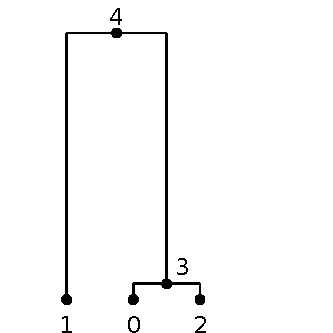
\includegraphics[width=0.4\textwidth]{images/plot_1.pdf}
\end{center}
\caption{\label{fig-simple-tree} Coalescent tree simulated by \msprime.
The tree is plotted using the \texttt{tree.draw\_svg()} method.}
\end{figure}

\begin{pythoncode}
import msprime
ts = msprime.sim_ancestry(2)
tree = ts.first()
tree.draw_svg()
\end{pythoncode}

This code chunk illustrates the basic approach required to draw a tree
in a Jupyter notebook. We first generate a tree sequence object (\texttt{ts}), sampling 2 individuals from,
and we then obtain the tree object representing the first (and only)
tree in this sequence. Finally, using the \texttt{draw\_svg()} method, we plot
the tree in SVG format. Another way to draw the tree is to use the
\texttt{draw\_text()} method. This method prints the tree to the console
as a string, which could be a very useful debugging tool.
All code chunks in this chapter are included in the accompanying Jupyter
notebook and are fully runnable.

The output of one random realisation of this process is shown in
Figure~\ref{fig-simple-tree}. The resulting tree has 7 nodes:
nodes 0, 1, 2, and 3 are \emph{leaves} and
represent our samples. Note here that 2 samples gave 4 nodes;
that's because the default ploidy in \msprime\ is diploid.
More details about ploidy in \msprime\ are in section~\ref{ploidy}.
Node 4 is an \emph{internal} node and is the
parent of 1 and 3. Similarly, Node 5 is an internal node and is the
parent of 0 and 2. Node 6 is also an internal node and is the root of
the tree. In \msprime, we always refer to nodes by their integer IDs and
obtain information about these nodes by calling methods on the tree
object. For example, the code \texttt{tree.children(6)} will return the
tuple \texttt{(4,\ 5)} here, as these are the node IDs of the children
of the root node. Similarly, \texttt{tree.parent(0)} will return
\texttt{5}.

The height of a tree node is determined by the \emph{time} at which the corresponding
ancestor was born. So,
contemporary samples always have a node time of zero, and time values
increase as we go upwards in the tree (i.e.\ further back in time). Times
in \msprime\ are always measured in \emph{generations}.

When we run a single simulation, the resulting tree is a single random
sample drawn from the probability distribution of coalescent trees. Since a
single random draw from any distribution is usually uninformative, we
nearly always need to run many different \emph{replicate} simulations to
obtain useful information. This simplest way to do this in \msprime\ is to
use the \texttt{num\_replicates} argument.

\begin{pythoncode}
import msprime
N = 1000
mean_T_mrca = 0
for ts in msprime.sim_ancestry(10, num_replicates=N):
    tree = ts.first()
    mean_T_mrca += tree.time(tree.root)
mean_T_mrca = mean_T_mrca / N
print(mean_T_mrca)

>>> 3.8478294094510166
\end{pythoncode}

    In this example we run 1000 independent replicates of the coalescent for
a sample of 10 chromosomes, and compute the mean time to the MRCA of the entire sample, i.e., the root of the
tree. The value of 3.85 generations in the past we obtain is of course highly unrealistic.
However, by default, time is measured in units of \(4 N_e\) generations (see the section~\ref{Demography}
for details on how to specify population models and interpret times). It is important to note here
that although time is measured in units of generations, this is of course
an approximation and we may have fractional values. Internally,
during a simulation time is scaled into coalescent units
using the \texttt{population\_size} parameter and once the
simulation is complete, times are scaled back into units of generations
before being presented to the user. This removes the burden of such
tedious time scaling calculations from the user. We discuss these time
scaling issues in more detail in the next section.

The
\texttt{sim\_ancestry} function behaves slightly differently when it is
called with the \texttt{num\_replicates} argument: rather than returning
a single tree sequence, we return an \emph{iterator} over the individual
replicates. This means that we can use the
convenient \textbf{for} loop construction to consider each simulation in
turn, but without actually storing all these simulations. As a result,
we can run millions of replicates using this method without
using any extra storage.

When simulating coalescent trees, we are often interested in more than
just the mean of the distribution of some statistic. Rather than compute
the various summaries by hand (as we have done for the mean in the last
example), it is convenient to store the result for each
replicate in a NumPy array and analyse the data after the simulations have completed.
For example:

\begin{pythoncode}
import msprime
import numpy as np
N = 1000
T_mrca = np.zeros(N)
for j, ts in enumerate(
        msprime.sim_ancestry(10, num_replicates=N)):
    tree = ts.first()
    T_mrca[j] = tree.time(tree.root)
print([np.mean(T_mrca), np.var(T_mrca)])

>>> (np.float64(3.836115509145935), np.float64(5.046041442780643))
\end{pythoncode}

    Here we simulate 1000 replicates, storing the time to the MRCA for each replicate in the array \texttt{T\_mrca}.  We use the Python \texttt{enumerate} function to simplify the process of efficiently inserting values into this
array, which simply ensures that \texttt{j} is \texttt{0} for the first replicate,
\texttt{1} for the second, and so on. Thus, by the time we finish the
loop, the array has been filled with $T_{MRCA}$ values generated
under the coalescent. We then use the NumPy library (which has
an extensive suite of statistical functions) to compute the mean and
variance of this array. This example is idiomatic, and we will use this
type of approach throughout. In the interest of brevity, we will omit all
further \texttt{import} statements from code chunks.

It is usually more convenient to use the \texttt{num\_replicates}
argument to perform replication, but there are situations in which it is
desirable to specify random seeds manually. For example, if simulations
require a long time to run, we may wish to use multiple processes to
run these simulations. To ensure that the seeds used in these different
processes are unique, it is best to manually specify them. For example,

\begin{pythoncode}
import concurrent.futures as cf

def run_simulation(seed):
    ts = msprime.sim_ancestry(10, random_seed=seed)
    tree = ts.first()
    return tree.time(tree.root)

N = 1000
seeds = np.random.randint(1, 2**32 - 1, N)
with cf.ProcessPoolExecutor(max_workers=4) as executor:
    futures = [
        executor.submit(run_simulation, seed) for seed in seeds]
    T_mrca = np.array([
        f.result() for f in cf.as_completed(futures)])
print(np.mean(T_mrca))

>>> np.float64(3.795412873593211)
\end{pythoncode}

    In this example we create a list of 1000 seeds between 1 and $2^{32} -
1$ (the range accepted by \msprime) randomly. We then use the
concurrent.futures module to create a process pool of four workers, and
run our different replicates in parallel. The results are then
collected together in an numpy array so that we can easily process them.
This approach is a straightforward way to utilise modern
multi-core processors.

Specifying the same random seed for two different simulations (with the
same parameters) ensures that we get precisely the same results from
both simulations (at least, on the same computer and with the same
software versions). This is very useful when we wish to examine the
properties of a specific simulation (for example, when debugging), or if
we wish to illustrate a particular example. We will often set the random
seed in the examples in this tutorial for this reason.

\subsection{Mutations}\label{mutations}

We cannot directly observe gene genealogies; rather, we observe mutations in a sample of sequences which ultimately have occurred on genealogical branches. We are
therefore very often interested not just in the genealogies generated by the coalescent process, but also in the results of
mutational processes imposed on these trees. \msprime\ simulates mutations using the \texttt{sim\_mutations} function. In its simplest form, this function takes
a tree sequence object and a \texttt{rate} parameter, then it returns a new tree sequence object with mutations added. This \texttt{rate} parameter specifies the
per-generation per-site mutation rate. For example, the following code chunk simulates a tree with mutations:

\begin{figure}[t]
\begin{center}
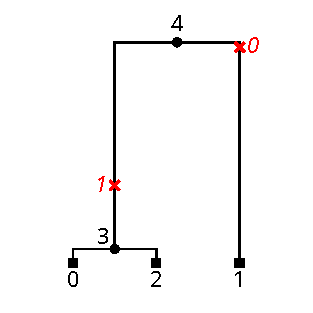
\includegraphics[width=0.4\textwidth]{images/plot_2.pdf}
\end{center}
\caption{\label{fig-tree-mutations} Coalescent tree with mutations}
\end{figure}

\begin{pythoncode}
ts = msprime.sim_ancestry(
    2, random_seed=13, sequence_length=10)
ts = msprime.sim_mutations(ts, rate=0.01, random_seed=2)
tree = ts.first()
tree.draw_svg()
\end{pythoncode}

As this code chunk suggests, simulating mutations on a tree sequence is a two-step process.
First, we simulate the genealogy using \texttt{sim\_ancestry} and store the resulting
tree sequence in the variable \texttt{ts}. Note that we specified a \texttt{sequence\_length} parameter;
this will specify the number of discrete sites in the sequence. After that, in the second
line, we simulate mutations on this tree sequence using the \texttt{sim\_mutations} function.
We specified a \texttt{rate} parameter for the \texttt{sim\_mutations} function; this
parameter specifies the per-generation per-site mutation rate. We overwrote the \texttt{ts} variable
with the new tree sequence object that now contains mutations to save memory, as otherwise we would
store the tree sequence twice in memory---once without mutations and once with mutations. We then
select the first and only tree in the tree sequence and plot it using the \texttt{draw\_svg()}
method. The tree produced by this code chunk is shown in Figure~\ref{fig-tree-mutations}.

As Figure ~\ref{fig-tree-mutations} shows, this code simulated two mutations, shown by the red "X"s.
Mutations occur above a given node in the tree, and all samples beneath
this node will inherit the mutation. The mutational model used here, which is the default mutational
model, is a Jukes-Cantor model (in the next section we will talk about other mutational models).
One convenient way to access the resulting sample genotypes is to loop through variants in the
tree sequence object. As each variant stores the position of the mutation, the alleles that are present
In the following code chunk, we investigate the mutations that have occurred in the previous simulation:

\begin{pythoncode}
for var in ts.variants():
    print(var.site.position, var.alleles, var.genotypes, sep="\t")
>>> 3.0	('A', 'T')	[0 1 0 1]
    9.0	('G', 'A')	[0 0 1 0]
\end{pythoncode}

Accessing genotype data is discussed in more detail in Section~\ref{processing-variants}.

\runinhead{Other mutation models} \

Beside the Jukes-Cantor model mentioned before, the \msprime\ mutation generation engine supports a list of mutation models; Table~\ref{tab:mutation-models}
lists these available models. These models include all the supported models by Seq-Gen~\citep{rambaut1997seq}, and they have been extensively tested against the
output of Seq-Gen~\citep{rambaut1997seq} and Pyvolve~\citep{spielman2015pyvolve} to ensure their accuracy. Moreover, \msprime\ allows for the specification of a custom mutation model—please refer
to the \msprime\ documentation for more in-depth information regarding creating a custom mutation model.

\begin{table}[h]
\centering
\begin{tabular}{|l|p{8cm}|}
\hline
\textbf{Name} & \textbf{Model} \\
\hline
BinaryMutationModel & Basic binary mutation model with two flip-flopping alleles : “0” and “1”. \\
\hline
JC69 & Jukes \& Cantor model~\citep{jukes1969evolution}, equal probability of transitions between nucleotides \\
\hline
HKY & Hasegawa, Kishino \& Yano model~\citep{hasegawa_1985_dating}, different probabilities for transitions and transversions \\
\hline
F84 & Felsenstein model~\citep{felsenstein1996hidden}, different probabilities for transitions and transversions \\
\hline
GTR & The Generalised Time-Reversible nucleotide mutation model~\citep{tavare1986some}, a general parameterisation of a time-reversible mutation process \\
\hline
BLOSUM62 & The BLOSUM62 model of time-reversible amino acid mutation~\citep{henikoff1992amino} \\
\hline
PAM & The PAM model of time-reversible amino acid mutation~\citep{dayhoff1978} \\
\hline
MatrixMutationModel & Superclass of the specific mutation models with a finite set of states \\
\hline
SMM & Stepwise mutation model for microsatellite repeat copy number~\citep{kimura_1978_stepwise} \\
\hline
TPM & Two-phase mutation model for microsatellite repeat copy number~\citep{dirienzo_1994_mutational} \\
\hline
EL2 & Two-phase mutation model, equal rate, linear bias model for microsatellite repeat copy number~\citep{garza_1995_microsatellite} \\
\hline
InfiniteAlleles & A generic infinite-alleles mutation model \\
\hline
SLiMMutationModel & An infinite-alleles model of mutation producing SLiM-style mutations \\
\hline
\end{tabular}
\caption{Mutation models supported by \texttt{msprime}.}
\label{tab:mutation-models}
\end{table}

To specify a mutation model, we pass the model to the \texttt{sim\_mutations} function using the \texttt{model} parameter. Some models
require additional parameters to be specified. For example, the \texttt{HKY} model requires the transitions/transversions ratio to be specified.
In the following code chunk, we simulate a tree with mutations using the \texttt{HKY} model:

\begin{pythoncode}
hky = msprime.HKY(kappa=0.75)
ts = msprime.sim_ancestry(5, random_seed=5, sequence_length=1e6)
ts = msprime.sim_mutations(
    ts, rate=1e-6, model=hky, random_seed=7)
\end{pythoncode}

In this example, we first specified the mutational model in the first line as the \texttt{HKY} model. In this model, the \texttt{kappa} parameter specifies
the transitions/transversions ratio. We then simulated a tree sequence with a sequence length of 1 million sites. After that we simulated mutations on this tree
sequence using the \texttt{HKY} model we specified with a mutation rate of \(10^{-6}\) per site per generation.

\runinhead{Scaled mutation rate} \

When comparing simulations to analytic results, it is very important to be aware of the way in which the
mutation rates are defined in coalescent theory. For historical reasons,
the scaled mutation rate \(\theta\) is defined as \(2N_e \mu\), where
\(\mu\) is the per-generation mutation rate. Since all times and rates
are specified in units of generations in \msprime, we must divide by a
factor of two if we are to compare with analytic predictions. For
example, the mean number of segregating sites for a sample of two is
\(\theta\); to run this in \msprime\ we do the following:

\begin{pythoncode}
N = 10000
theta = 5
S = np.zeros(N)
replicates = msprime.sim_ancestry(2, population_size=1,
    num_replicates=N, ploidy=1, discrete_genome=False)
for j, ts in enumerate(replicates):
    ts = msprime.sim_mutations(
        ts, rate=theta/2, discrete_genome=False)
    S[j] = ts.num_sites  # Number of segregrating sites.

print(np.mean(S))

>>> np.float64(5.0281)

\end{pythoncode}

    Note that here we set the mutation rate to \(\theta / 2\) (to cancel out
the factor of 2 in the definition of \(\theta\)) and \emph{ploidy = 1} (so
that time is measured in haploid coalescent time units; the following section discusses the ploidy parameter in more detail). Such
factor-of-two gymnastics are unfortunately unavoidable in coalescent
theory.

\subsection{Demography}\label{Demography}

\subsubsection{Population size}\label{population-models}

In the previous section the only parameters we supplied to
\texttt{sim\_ancestry} were the \texttt{sample\_size} and
\texttt{num\_replicates} parameters. This allows us to randomly sample
trees with a given number of nodes, but, as it leaves the population
unspecified, has little connection with
biological reality. The most fundamental population parameter is the \emph{effective population size}, or
\(N_e\). This parameter simply rescales time; larger effective
population sizes correspond to older coalescence times. The following code chunk
calculates a mean pairwise coalescence time for a sample of size 2 for different
population sizes:

\begin{pythoncode}
def pairwise_T_mrca(population_size, ploidy):
    N = 10000
    T_mrca = np.zeros(N)
    for j, ts in enumerate(msprime.sim_ancestry(2,
            population_size=population_size,
            num_replicates=N, ploidy=ploidy)):
        tree = ts.first()
        T_mrca[j] = tree.time(tree.root)
    return np.mean(T_mrca)

print(
    pairwise_T_mrca(1, ploidy=1), pairwise_T_mrca(10, ploidy=1),
    pairwise_T_mrca(100, ploidy=1))

>>> (np.float64(0.9965894759060011),
     np.float64(10.036428076042618),
     np.float64(99.25331259141007))

\end{pythoncode}

    Thus, when we specify \emph{population\_size=10} we get a mean pairwise coalescence time of about
10 generations, and with \emph{population\_size=100}, the mean coalescence time is about
100 generations (when we simulate haploids). See \cite{wakely2008coalescent} for details on the
biological interpretation of effective population size.

\runinhead{Ploidy and timescale}\label{ploidy} \

The \texttt{sim\_ancestry} function accepts a ploidy parameter. Theoretically, ploidy referes the number of genomes per individual.
In \msprime, the ploidy parameter determines the number of nodes per sample, and it scales time accordingly.

By default, \emph{population\_size=1} in \msprime, which is equivalent to measuring
time in units of \(N_e\) generations. It is very important to note that
\texttt{population\_size} in \msprime\ is the \emph{ploidy} effective population size,
which means that by default, all times are scaled by \(2N_e\), since the default ploidy is diploid. Similarly, however,
if we set ploidy to 1, i.e., simulating haploids, time will be scaled by $N_e$. Thus, care about ploidy
and population size is required when comparing results from \msprime\ with expectations from the literature, which
are generally given in diploid coalescent time units. For example, we know that the expected
coalescence time for a sample of size 2 is 1, and this is the value we
obtain from the \texttt{pairwise\_T\_mrca} function when we set \emph{population\_size=1}, since \emph{ploidy}
is set to 1. To obtain the same result for a diploid population, where ploidy is set to 2, first, we need to set
sample size to 1 since we will get two nodes per sample instead of one node per sample. And second, we need to set population
size to 0.5, as coalescence time is scaled by \(2N_e\) instead of \(N_e\).

We will usually assume that we are working in haploid
coalescent time units from here on and so set \emph{population\_size=1} and \emph{ploidy=1} in most
examples. However, when running simulations of a specific organism and/or population, it
is substantially more convenient to use an appropriate estimated value
for \emph{population\_size} so that times are directly interpretable.

\runinhead{Exponentially growing/shrinking
populations}\label{exponentially-growingshrinking-populations} \

When we provide a \emph{population\_size} parameter, this specifies a fixed effective
population size. We can also model populations that are exponentially
growing or contracting at some rate over time. Given a population size
at the present \(s\) and a growth rate \(\alpha\), the size of the
population \(t\) generations in the past is $s e^{-\alpha t}$. (Note
again that time and rates are measured in units of \emph{generations},
not coalescent units.)

In \msprime, the initial size and growth rate for a particular population
are specified using a \texttt{Demography} object. A \texttt{Demography} object
(describing the different populations; see Section~\ref{population-structure})
is then provided to the \texttt{sim\_ancestry} function. When providing a
\texttt{Demography} object, setting a \texttt{population\_size} to
\texttt{sim\_ancestry} is not required, as the \texttt{initial\_size} of the
\texttt{Demography} object performs the same task. For example,

\begin{pythoncode}
def pairwise_T_mrca(growth_rate):
    N = 10000
    T_mrca = np.zeros(N)
    demography = msprime.Demography()
    demography.add_population(
        initial_size=1, growth_rate=growth_rate)
    replicates = msprime.sim_ancestry(
        samples=2, demography=demography,
        num_replicates=N, random_seed=16)

    for j, ts in enumerate(replicates):
        tree = ts.first()
        T_mrca[j] = tree.time(tree.root)
    return np.mean(T_mrca)

print(
    pairwise_T_mrca(0.05), pairwise_T_mrca(0),
    pairwise_T_mrca(-0.05))
>>> (np.float64(1.8619023833007429),
     np.float64(2.0358305242092154),
     np.float64(2.3064938769701295))
\end{pythoncode}

    Here we simulate the pairwise \(T_{MRCA}\) for positive, zero and
negative growth rates. When we have a growth rate of zero, we see that we
recover the usual result of 2.0—as our ploidy-scaled initial size (two genomes x one individual), and hence \emph{population\_size},
is set to 1 diploid individual. When the growth rate is positive, we see that the
mean coalescence time is reduced, since the population size is getting
smaller as we go backwards in time, resulting in an increased rate of
coalescence. Conversely, when we have a negative growth rate, the
population is getting larger as we go backwards in time, resulting in a
slower coalescence rate. (Care must be taken with negative growth rates,
however, as it is possible to specify models in which the MRCA is never
reached. In some cases this will lead to an error being raised, but it
is also possible that the simulator will keep generating events
indefinitely. This is particularly important in simulation based
approaches to inference from real data.)


\subsubsection{Population structure}\label{population-structure}
To facilitate population structure modelling, \msprime\ implements
predefined theoretical models. The simplest model is the isolated model,
where populations are simulated in isolation, i.e., without migration.

\runinhead{Isolated model}\label{isolated-model} \

The method \texttt{msprime.Demography.isolated\_model()} is used to
simulate populations in isolation. The \texttt{initial\_size} parameter
specifies the initial population size, and the \texttt{growth\_rate}
parameter specifies the growth rate of the population. Both parameters
are lists, where each element corresponds to a population. In the
following line, we set up a simple model of two populations in isolation:
\begin{pythoncode}
    demography = msprime.Demography.isolated_model(
        [1, 1], growth_rate=[0.01, 0.02])
\end{pythoncode}
Although the two populations are simulated without migration, we can
specify migration rates between populations using the \texttt{set\_migration\_rate()}
method. This method takes the source and destination populations and the migration rate as arguments.
To add migration between populations 0 and 1, we use the following line:
\begin{pythoncode}
    demography.set_migration_rate(source=0, dest=1, rate=0.1)
\end{pythoncode}

In this line, the \texttt{source} argument specifies the source population from which lineages originate. The
\texttt{dest} argument specifies the destination population to which lineages migrate. The \texttt{rate} argument
specifies the per-generation migration rate between the source and destination populations.

Note that the migration rate defined by \msprime\ is the lineage migrationn rate, not the individual
migration rate: While the individual migration rate is the proportion of individuals in the source
population that migrate to the destination population in each generation, the lineage migration rate
is defined as this proportion (individual migration rate) multiplied by the ratio between the source
population size and the destination population size. Please refer to the \msprime\ documentation for
more information on the migration rate.

\runinhead{Island model}\label{island-model} \

When the migration rate is the same between simulated populations, we don't
need to specify the migration rate between each pair of populations. Instead,
we can use the \texttt{island\_model()}. The \texttt{Demography.island\_model()} accepts
the same parameters as the \texttt{Demography.isolated\_model()} method in
addition to the \texttt{migration\_rate} parameter. The following line sets up an
\texttt{island\_model()} with three populations:
\begin{pythoncode}
    demography = msprime.Demography.island_model(
        [1, 1, 1], migration_rate=0.1)
\end{pythoncode}

This single line is equivalent to setting up an isolated model with three populations
and setting up migration rate of 0.1 between each pair of populations.

\runinhead{Stepping stone model}\label{stepping-stone-model} \

Similar to the \texttt{island\_model()}, the \texttt{stepping\_stone\_model()}
accepts a single migration rate parameter. However, the stepping stone model simulates
migration between adjacent populations exclusively. This model considers populations to be
adjacent in a linear fashion.

\subsubsection{Demographic events}\label{demographic-events}

Demographic events allow us to model more complex histories involving
changes to the population structure over time and are specified using
a \texttt{demography} object. Each
demographic event occurs at a specific time, and we recommend specifying them
in the order they occur (backwards in time). There are a
number of different types of demographic events that msprime supports, for example
\texttt{add\_population\_parameters\_change()} changes the growth rate or size of a population;
\texttt{add\_population\_split()} simulates a scenario where a population is derived from a
specific population at a certain time (split event);
and \texttt{add\_admixture()} simulates a population admixture event, where a population is
formed by the admixture of two or more populations.

\begin{figure}[t]
\centering
% \qquad
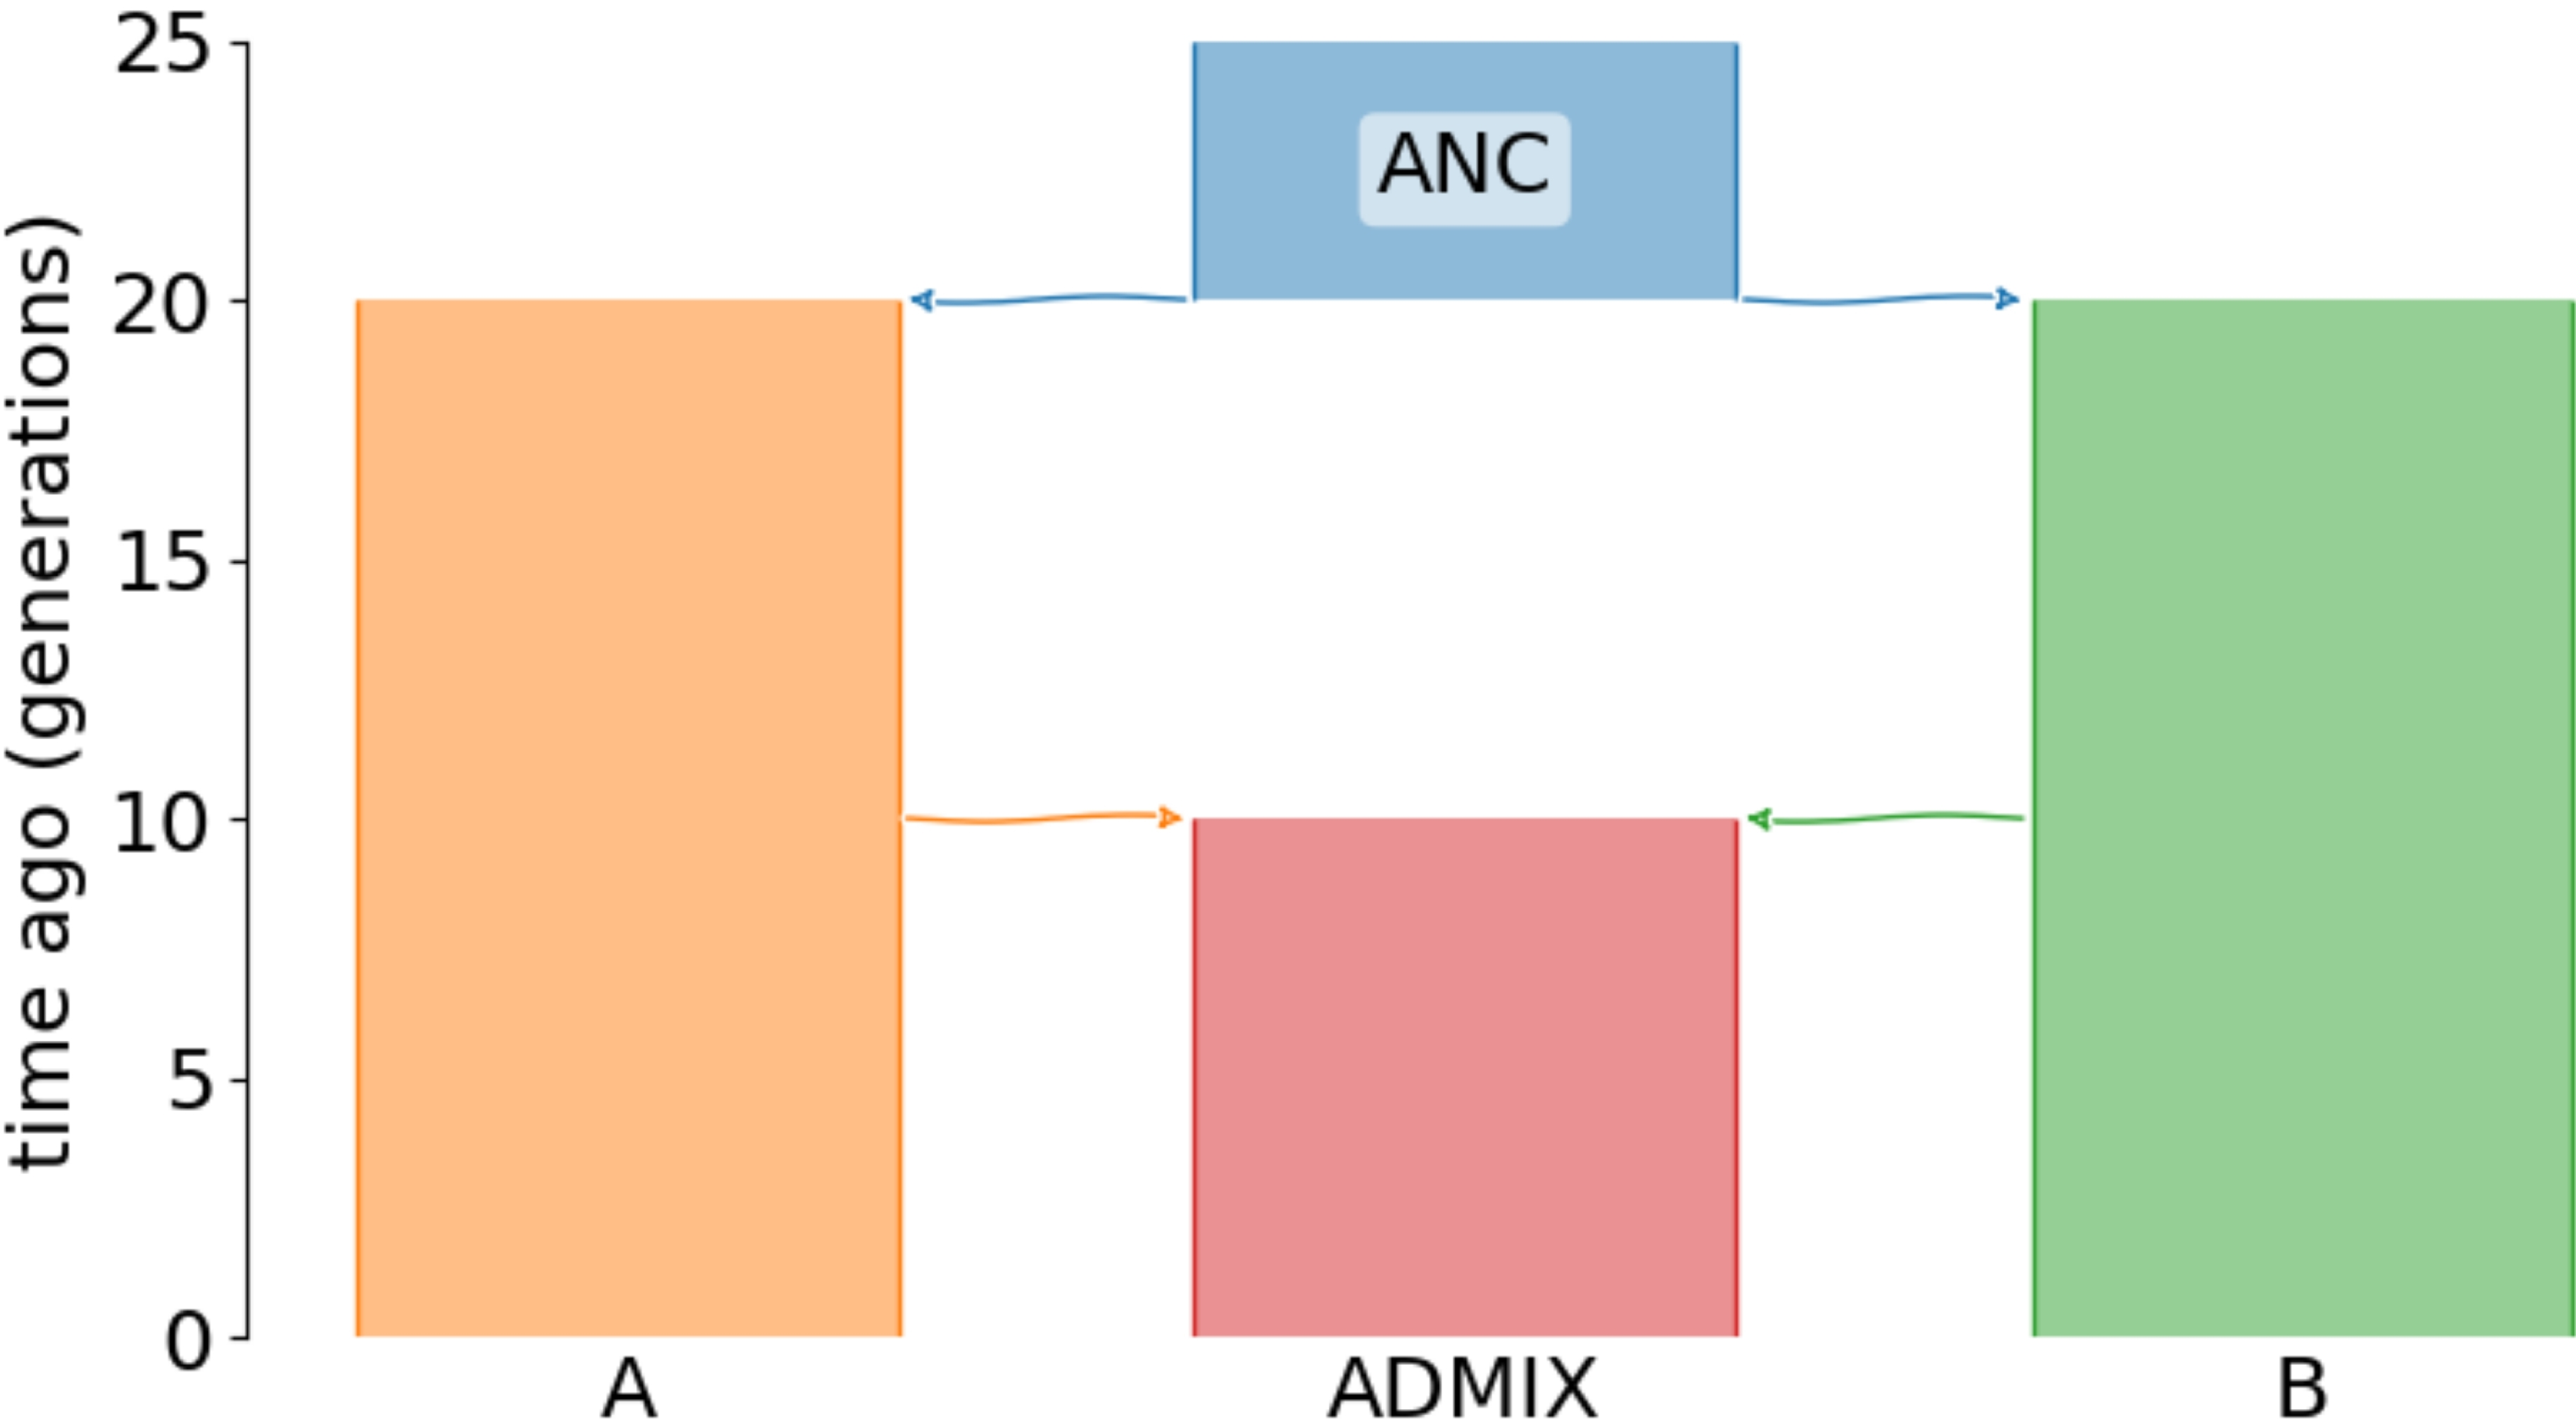
\includegraphics[width=0.75\textwidth]{images/admixture.pdf}
\caption{\label{fig:complex-demography}An example of a complex demography that could be
simulated using \msprime. This figure is generated by expressing demography using the
\texttt{Demes} standard format and plotted using the \texttt{demesdraw} package.}
\end{figure}

\runinhead{Complex demography}\label{Complex-demography} \

To simulate complex demography, we use the \texttt{Demography} class to specify different
demographic events that make this complex model. In the following example, we will
simulate an ancestral population (ANC) that splits into two populations (A and B) at time
20 generations ago. After 10 generations, populations A and B admix with proportions of 0.25
and 0.75, respectively, to form population (ADMIX). Figure~\ref{fig:complex-demography}
illustrates this model.

\begin{pythoncode}
    demography = msprime.Demography()
    demography.add_population(name="A", initial_size=100)
    demography.add_population(name="B", initial_size=100)
    demography.add_population(name="ADMIX", initial_size=100)
    demography.add_population(name="ANC", initial_size=100)
    demography.add_admixture(
        time=10, derived="ADMIX", ancestral=["A", "B"],
        proportions=[0.25, 0.75])
    demography.add_population_split(
        time=20, derived=["A", "B"], ancestral="ANC")
\end{pythoncode}

In this example, we use the \texttt{add\_population()} method to add the four populations
to the model. The method \texttt{add\_admixture()} is used to specify the admixture event;
this method takes the time of the event, the name of the derived population, the ancestral
populations, and the proportions of each ancestral population in the derived population.
The method \texttt{add\_population\_split()} is used to specify the population split event;
similar to the \texttt{add\_admixture()} method, it takes the time of the event, the derived
populations, and the ancestral population.

Simulating this model using the \texttt{sim\_ancestory} function is straightforward:
\begin{pythoncode}
ts = msprime.sim_ancestry(
    samples={"A":1, "B":1, "ADMIX":1}, demography=demography)
\end{pythoncode}

In this line, we pass a dictionary as the \texttt{samples} parameter to the \texttt{sim\_ancestry} method to
specify the number of samples drawn from each population. Here, we draw one sample from each of the populations
\emph{A}, \emph{B}, and \emph{ADMIX}. The \texttt{demography} object that was set up in the previous code chunk
is passed to the \texttt{sim\_ancestry} function to simulate the tree sequence under this complex demography.

\runinhead{Demography debugger}\label{demography-debugger}\

Keeping track of complex models can be challenging, and \msprime, for this reason,
provides the \texttt{DemographyDebugger} class. This class provides a visual summary of
the demographic history by splitting time into epochs and displaying the demographic
events that take place in each epoch. In the previous example, to use the \texttt{DemographyDebugger} class,
we simply use \texttt{demography.debug()}, which displays the demographic history in an \texttt{HTML}
format. Figure~\ref{fig:DemographyDebugger} shows the \texttt{demography.debug()} output for the example in section~\ref{Complex-demography}.

\begin{figure}[t]
\centering
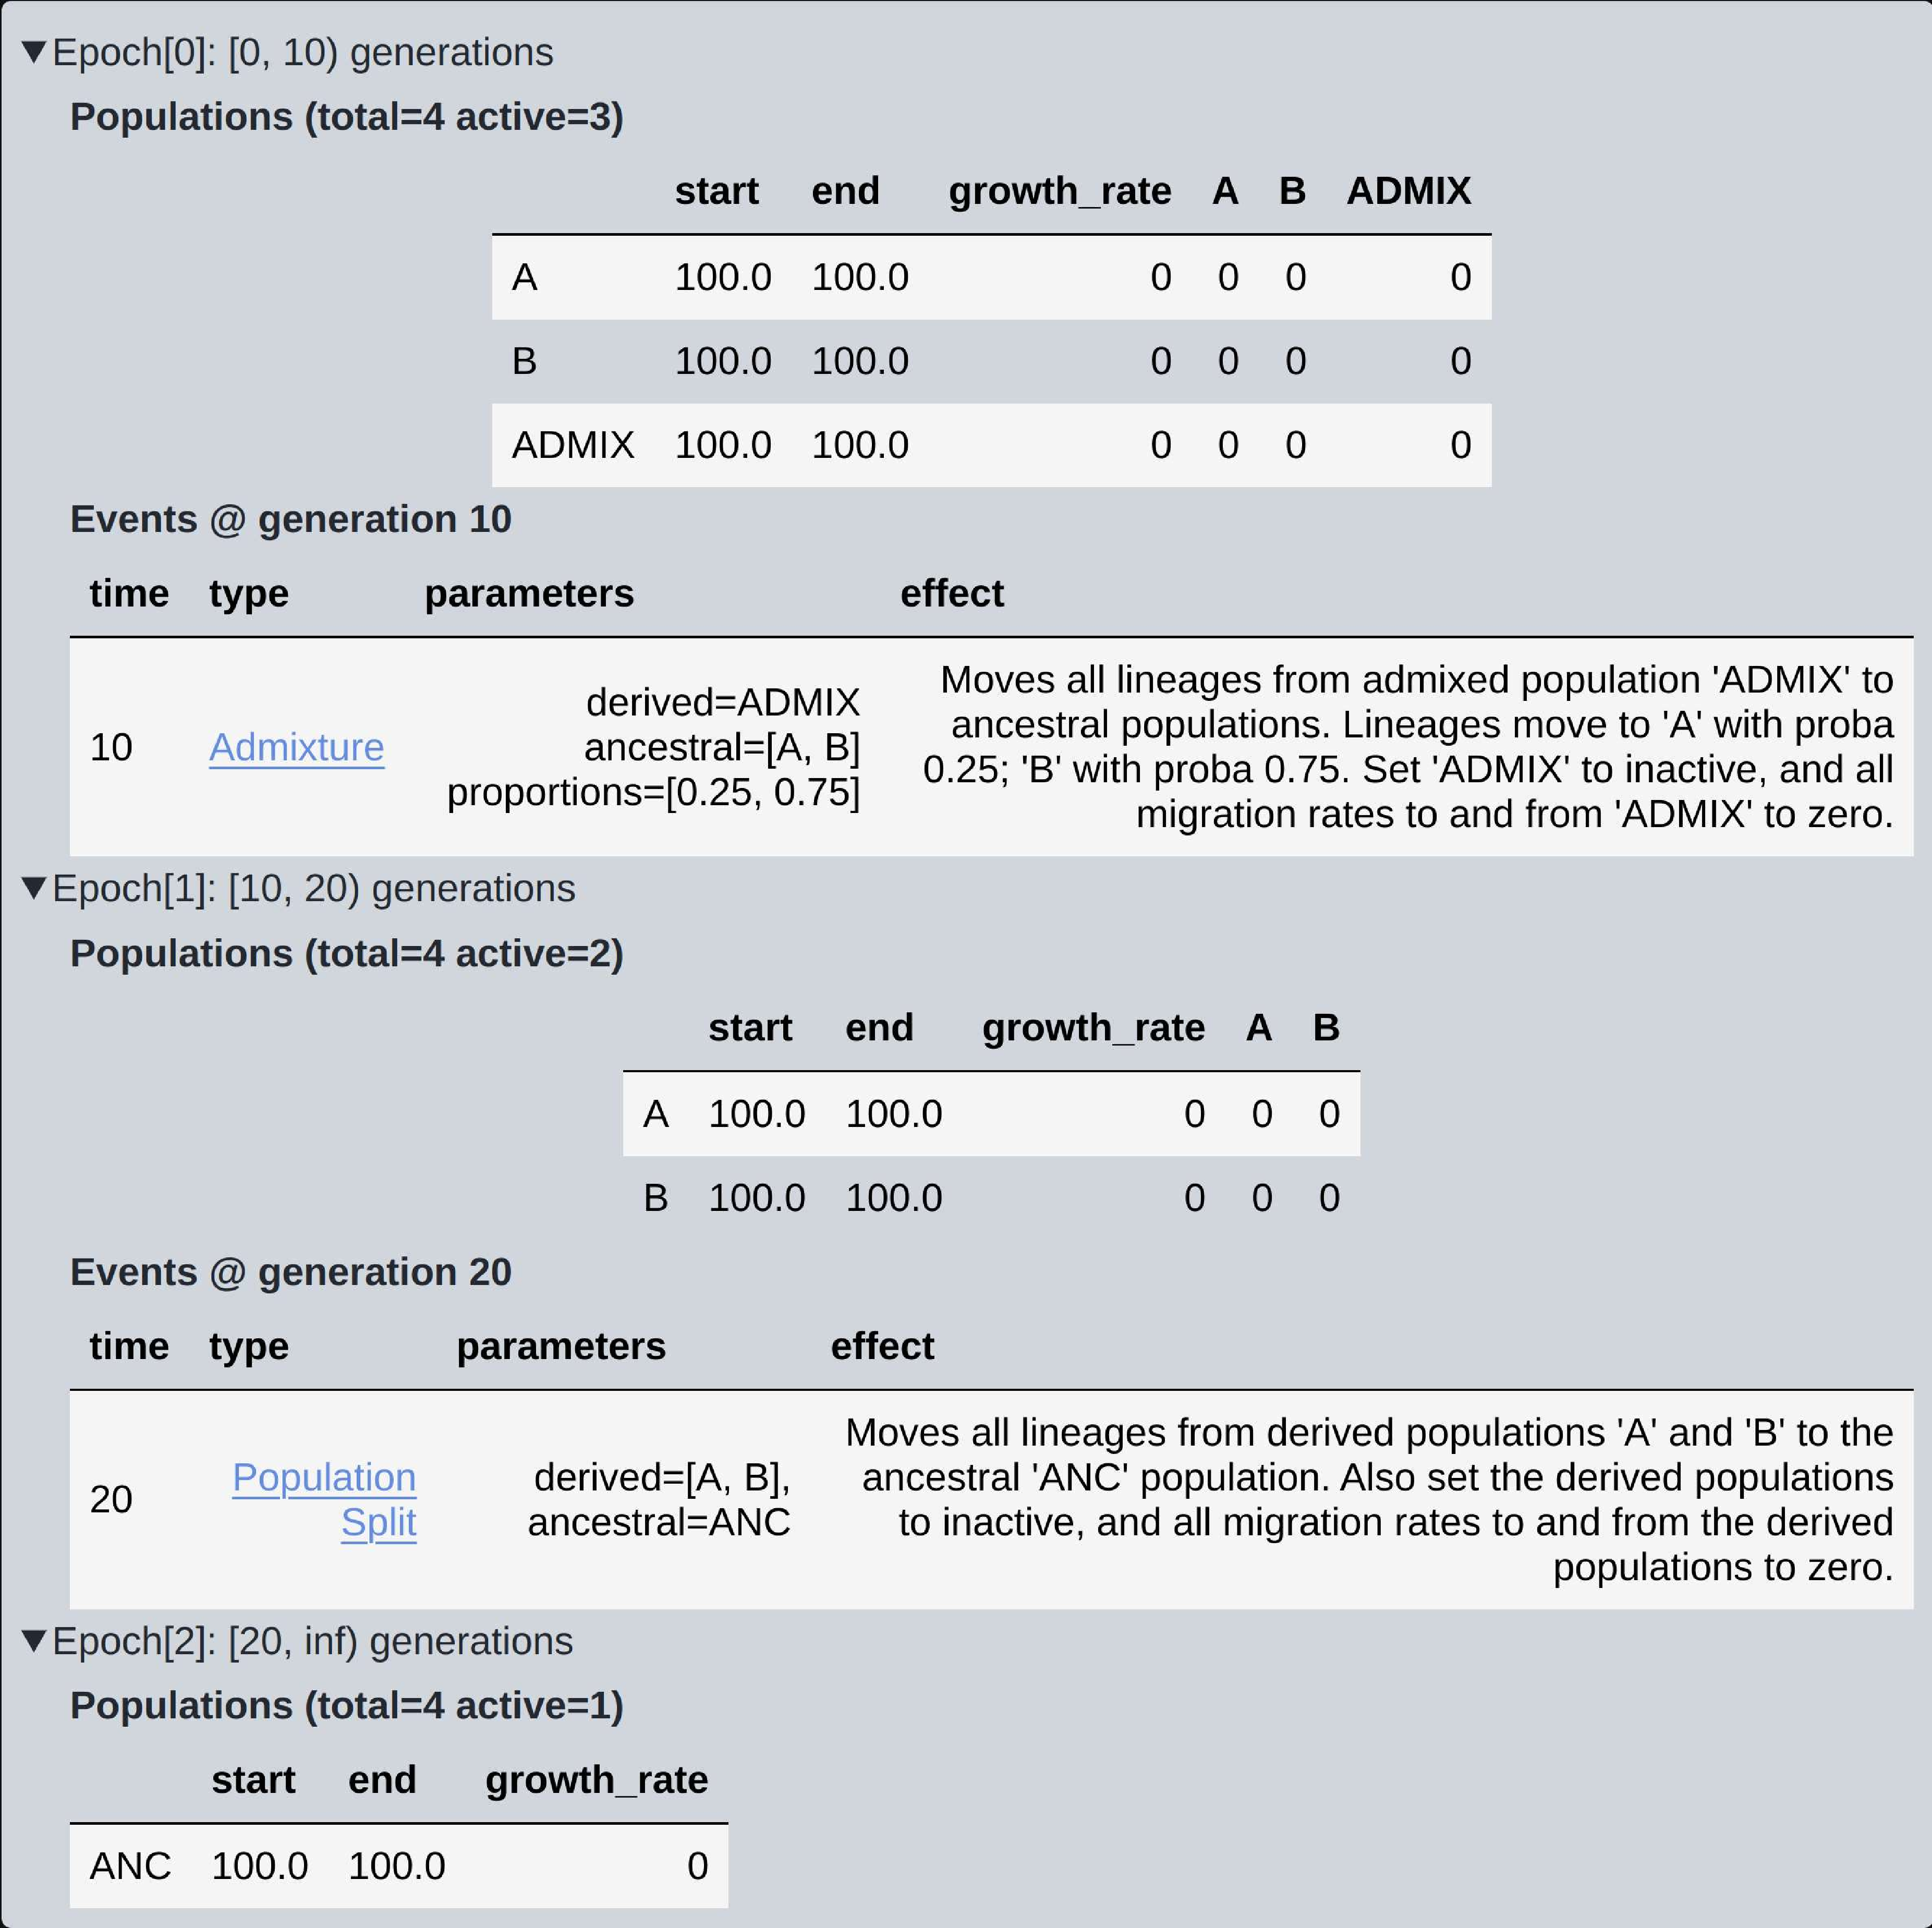
\includegraphics[width=\textwidth]{images/demography_debugger.pdf}
\caption{\label{fig:DemographyDebugger}The \texttt{DemographyDebugger} output for a complex demography.}
\end{figure}

\subsubsection{Using Demes standard format}\label{using-demes-standard-format}

The Demes format~\citep{gower2022demes} is a standard for writing
demographic models, to facilitate interchange between simulators, as well as between
demographic inference software and simulators. Demes models are typically written as a
YAML file, and loaded into Python using the demes library.

For example, the complex demography model described in section~\ref{Complex-demography} can be
written in the Demes format as follows:

\begin{footnotesize}
\begin{minted}{yaml}
time_units: generations
defaults:
    {epoch: {start_size: 100}}
demes:
    - {name: ANC, epochs: [{end_time: 20}]}
    - {name: A, ancestors: [ANC]}
    - {name: B, ancestors: [ANC]}
    - {name: ADMIX, ancestors: [A, B],
        proportions: [0.25, 0.75], start_time: 10}
\end{minted}
\end{footnotesize}

This YAML file can be loaded into Python using the demes library and can be represented
easily using the \texttt{demesdraw} package. The following code chunk demonstrates how to
load the Demes model from the YAML file and visualise it using \texttt{demesdraw}:

\begin{pythoncode}
graph = demes.load("admixture.yaml")
demesdraw.tubes(graph)
\end{pythoncode}

This code chunk produces Figure~\ref{fig:complex-demography}. In this figure, arrows indicate
the movement of individuals as time proceeds from the past to the present.


To import demes from a YAML file, we can use the \texttt{demes.load()} function to
load a demes graph object. Then, the \texttt{Demography.from\_demes()} method is used to convert a
\texttt{demes graph} object into a \texttt{Demography} object. On the
other hand, the \texttt{Demography.to\_demes()} method performs the opposite conversion; it
converts a \texttt{Demography} object to a \texttt{demes graph} object, which can then be
exported as a YAML file.

For example:

\begin{pythoncode}
import demes
graph = demes.load("admixture.yaml")
demography = msprime.Demography.from_demes(graph)
ts = msprime.sim_ancestry(
    {"A":2, "B":3, "ADMIX":2},
    demography=demography, random_seed=1234)
\end{pythoncode}

The previous code block loads the example demes model of Figure~\ref{fig:complex-demography} from a YAML file. Then, a demography
object is created from the loaded deme graph. Finally, a tree is simulated using the demography object, with samples
drawn from demes A, B, and ADMIX.


\subsubsection{Drawing samples}\label{ancient-samples}

The samples drawn from a simulation can be defined in one of three ways: by
simply providing an integer as the number of samples drawn from a single population,
by providing a dictionary with population names as keys and the number of
samples as values, or by providing a list of \texttt{SampleSet} objects.
An \msprime\ \texttt{SampleSet} object can be used to specify the sampling
time, the population, and the ploidy of a set of samples, making it the more
versatile option. However, in most cases, it is sufficient to define samples
using an integer or a dictionary.

Up to this point we have assumed that all samples are taken at the
present time. However, \msprime\ allows us to specify arbitrary sampling
times and locations, allowing us to simulate (for example) ancient
samples.

\begin{pythoncode}
demography = msprime.Demography.island_model(initial_size=[1, 1],
    migration_rate=1)
ts = msprime.sim_ancestry(
    samples=[
        msprime.SampleSet(1, population=0, time=0),
        msprime.SampleSet(1, population=0, time=0),
        msprime.SampleSet(1, population=0, time=0),
        msprime.SampleSet(1, population=1, time=0.75),
        # Ancient sample in deme 1
    ],
    demography=demography, ploidy=1, random_seed=22)
tree = ts.first()
\end{pythoncode}

\begin{figure}[t]
\centering
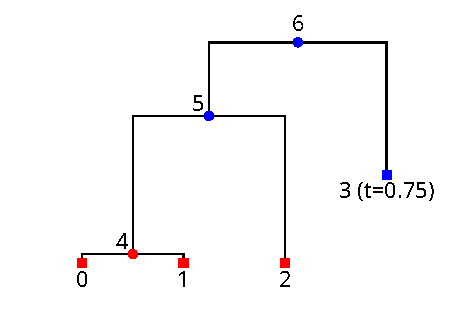
\includegraphics[width=0.48\textwidth]{images/plot_9.pdf}
\caption{\label{fig-tree-ancient-samples} Example tree produced by simulation
with ancient samples.}
\end{figure}

The tree produced by this code chunk is shown in Figure~\ref{fig-tree-ancient-samples}.
All of the trees that we previously considered had leaf nodes at time
zero. In this case, the samples 0, 1 and 2 are taken at time 0 from
population 0, but node 3 is sampled at time 0.75 from population 1.

Note that sampled individuals and nodes are defined sequentially based
on the order in which they are provided to the \texttt{samples} parameter. Also, it is vital
to note that changing the ploidy parameter only affects the number of samples drawn from
the population, not the actual simulation; simulations will be performed on the
haploid coalescent scale as set for the \texttt{sim\_ancestry} function; the ploidy of the simulation can be changed by changing the
\texttt{ploidy} parameter for the \texttt{sim\_ancestry} function.


\subsection{Recombination}\label{recombination}

One of the key innovations of \msprime\ is that it makes simulation of the
full coalescent with recombination possible at whole-chromosome scale.
Adding recombination to a simulation is simple, requiring very minor
changes to the methods given above.

\begin{pythoncode}
ts = msprime.sim_ancestry(
    10, population_size=1e4, sequence_length=1e5,
    recombination_rate=1e-8, random_seed=3)
print(ts.num_trees)
>>> 135
\end{pythoncode}

    In this case, we provide two extra parameters: \texttt{sequence\_length}, which
defines the length of the genomic region to be simulated, and
\texttt{recombination} \texttt{\_rate}, which defines the rate of recombination
per unit of sequence length, per generation. It is often useful to
think of both sequence lengths and recombination rates as defined in units of base-pairs.

For this example, we defined a sequence length of 100kb, and a recombination rate of
\(10^{-8}\) per base per generation. The result of this particular simulation is a
\emph{tree sequence} that contains 135 distinct trees. Other replicate
simulations with different random seeds will usually result in different
numbers of trees.

Up to this point we have focused on simulations that returned a single
tree representing the genealogy of a sample. The inclusion of
recombination, however, means that there may be more than one tree
relating our samples. The \texttt{TreeSequence} object returned by
\msprime\ is a very concise and efficient representation of these highly
correlated trees. To process the trees, we simply consider
them one at a time, using the \texttt{trees()} iterator.

\begin{pythoncode}
tmrca = np.zeros(ts.num_trees)
breakpoints = np.zeros(ts.num_trees)
for tree in ts.trees():
    tmrca[tree.index] = tree.time(tree.root)
    breakpoints[tree.index] = tree.interval[0]
plt.ylabel("T_mrca (Generations)")
plt.xlabel("Position (kb)")
plt.plot(breakpoints / 1000, tmrca, "o");
\end{pythoncode}

\begin{figure}
\begin{center}
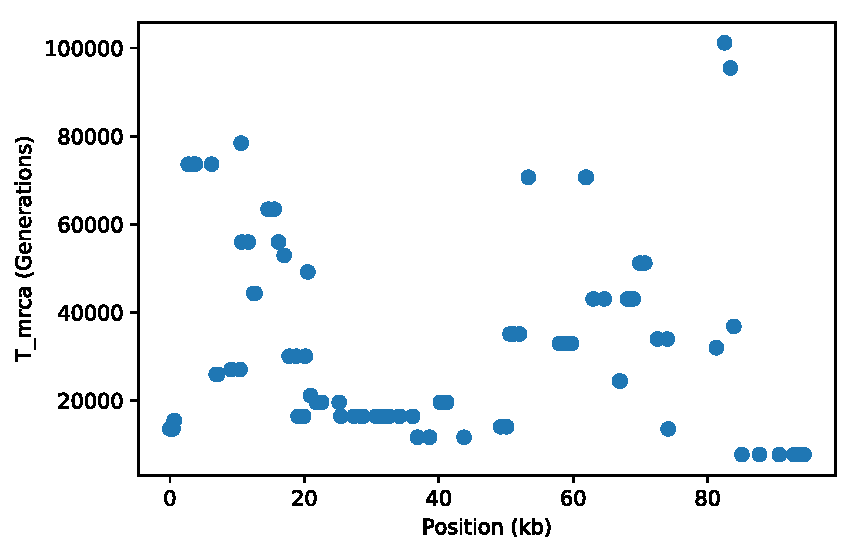
\includegraphics[width=\textwidth]{images/plot_10.pdf}
\end{center}
\caption{\label{fig:tree_tmrcas}Time to the MRCA of
a sample across a 100kb region.}
\end{figure}

This code generates the plot in Figure~\ref{fig:tree_tmrcas} showing the time of the MRCA of the sample for each tree across the
sequence. We find the \(T_{MRCA}\) as before, and plot this against the
left coordinate of the genomic interval that each tree covers. A full description of
\emph{tree sequences} and the methods for working with them is beyond the scope of this chapter (but see the online documentation for more details).

It is also possible to simulate data with recombination rates varying
across the genome (for example, in recombination hotspots). To do this, we
first create a \texttt{RecombinationMap} instance that describes the
properties of the recombination landscape that we wish to simulate. We
then supply this object to \texttt{sim\_ancestry} using the
\texttt{recombination\_map} argument. In the following example, we
simulate 100 samples using the human chromosome 22 recombination map
from the HapMap project~\citep{international2003international}.
Figure~\ref{fig:variable_recombination} shows the
recombination rate and the locations of breakpoints
from the simulation, and the density of breakpoints closely follows the
recombination rate, as expected.

\begin{pythoncode}
infile = "genetic_map_GRCh37_chr22.txt"
recomb_map = msprime.RateMap.read_hapmap(infile)
ts = msprime.sim_ancestry(
    samples=100, population_size=10**4,
    recombination_rate=recomb_map, ploidy=1, random_seed=1)
\end{pythoncode}

\begin{figure}
\begin{center}
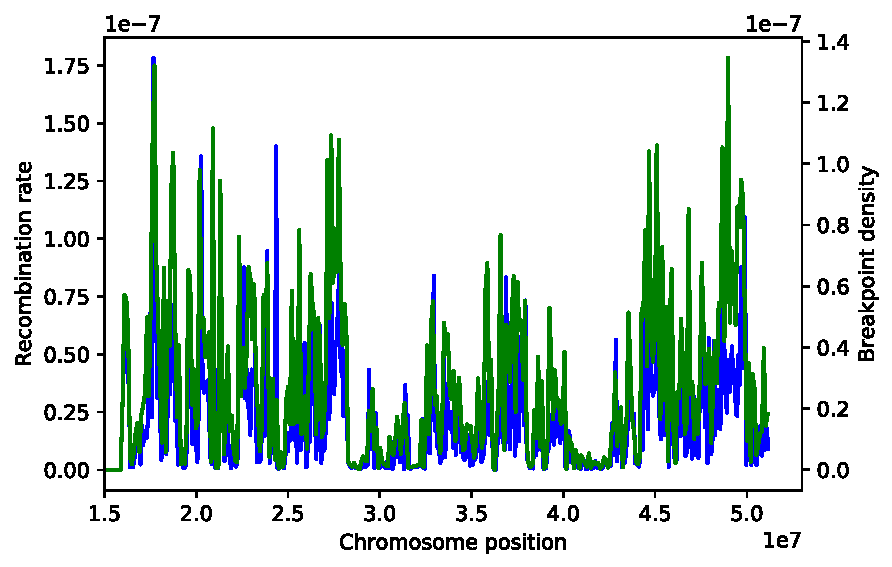
\includegraphics[width=\textwidth]{images/plot_11.pdf}
\end{center}
\caption{\label{fig:variable_recombination} The HapMap
genetic map for chromosome 22 (blue) matches the density of breakpoints for a simulated chromosome (green) well.}
\end{figure}

By default, \msprime\ simulates a discrete genome, where recombination
events occur at integer positions.

\begin{pythoncode}
recomb_map = msprime.RateMap.uniform(sequence_length=10, rate=1)
ts = msprime.sim_ancestry(2, recombination_rate=recomb_map)
print(list(ts.breakpoints()))
>>> [0, 1.0, 2.0, 3.0, 5.0, 6.0, 7.0, 8.0, 9.0, 10.0]
\end{pythoncode}

    Here we simulate the history of two samples in a system with 10 loci, each of
length 1 with a recombination rate of 1 between adjacent loci per
generation. In the output, we see that the breakpoints between trees now
occur exactly at the integer boundaries between these loci. It is also possible to simulate
a standard continuous genome by setting the \texttt{discrete\_genome} parameter for the \texttt{sim\_ancestry} function
to \texttt{False}.

\subsubsection{Gene conversion}\label{gene-conversion}

Beside simulating recombination, \msprime\ also supports gene conversion events. To simulate gene conversion,
two parameters are required: the gene conversion rate and the tract length distribution. By default, tract lengths are drawn
from a genometric distribution with a mean of 1.

Gene conversion can be simulated independently, or it can be simulated alongside recombination, provided that both rates are constants.
The following example shows a simulation with gene conversion and recombination.

\begin{pythoncode}
ts = msprime.sim_ancestry(
    3, gene_conversion_rate=0.02, gene_conversion_tract_length=1,
    sequence_length=10, random_seed=3)
\end{pythoncode}

\begin{figure}
\begin{center}
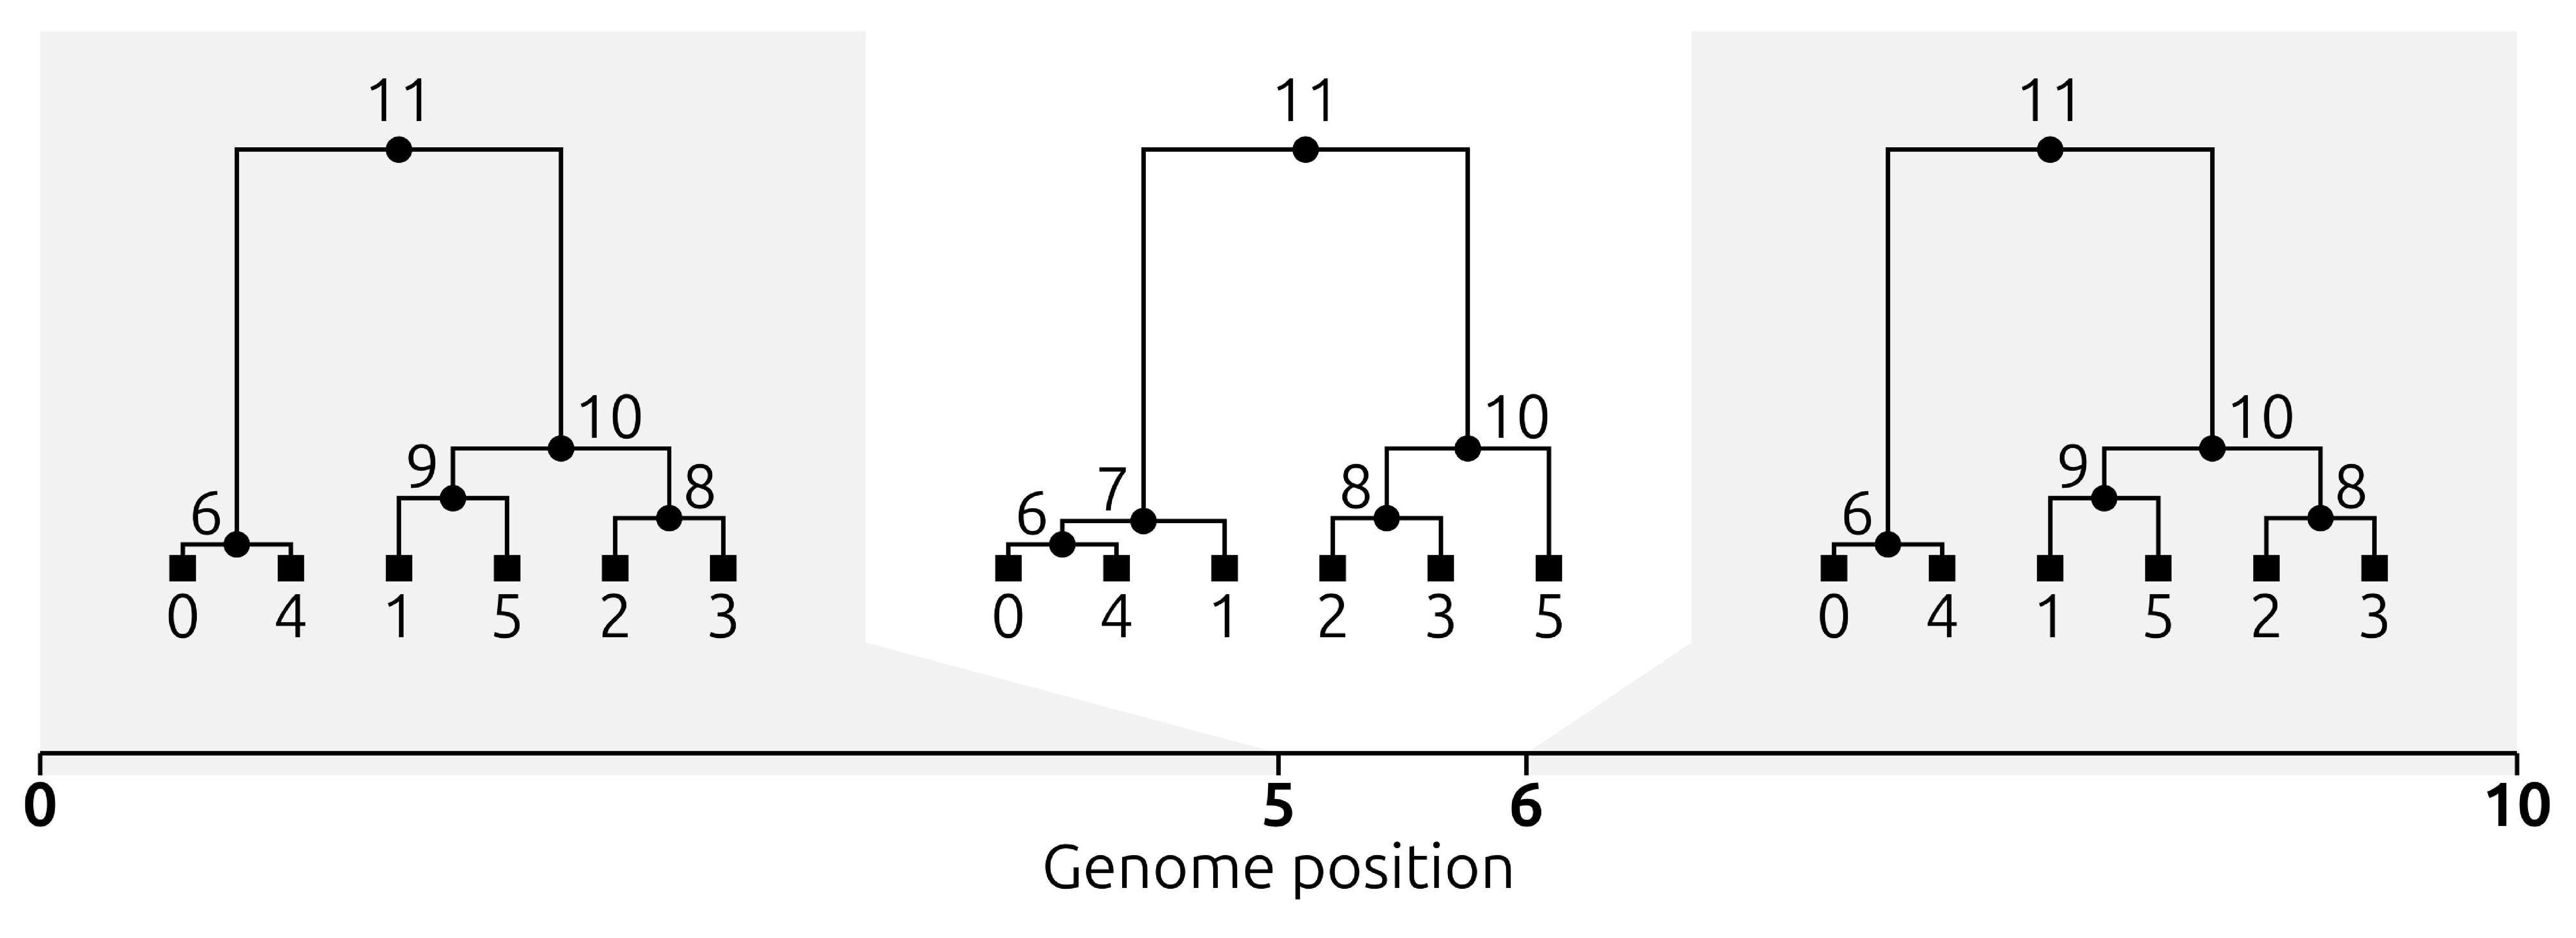
\includegraphics[width=\textwidth]{images/gene_conversion.pdf}
\end{center}
\caption{\label{fig:gene_conversion} An example of the effect of gene conversion on simulations.}
\end{figure}

In this example, as shown in Figure~\ref{fig:gene_conversion}, we see the gene conversion-specific effect; trees on either side of the event are identical.

\subsection{Ancestry Models}\label{ancestry-models}

By default, \msprime\ simulates the coalescent process based on the Hudson model \citep{hudson1983properties}, referred to as the
\emph{StandardCoalescent model}. However, \msprime\ is able to simulate the coalescent process using other models.

For large sample sizes and long recombining genomes, simulating recent human datasets, for example, the Hudson model can be
less accurate. In such cases, we recommend the use of the \emph{DiscreteTimeWrightFisher}~\citep{nelson2020accounting} model.
Since this model simulates the coalescence process generation-by-generation, it is less computationally efficient than the
Hudson model. Therefore, we recommend combining the two models as we will show in section~\ref{multiple-models}.

Sequentially Markov Coalescent (SMC) simulations are supported by \msprime\ in two models: the \emph{SmcApproxCoalescent}~\citep{mcvean2005approximating}
and the \emph{SmcPrimeApproxCoalescent}~\citep{marjoram2006fast}. These models, however, are only
recommended to study the SMC approximations, since they are not more accurate or less computationally expensive than the standard coalescent model.

Other models supported by \msprime\ include the \emph{BetaCoalescent}~\citep{schweinsberg03}, the \emph{DiracCoalescent}~\citep{BBE13},
the \emph{FixedPedigree} (discussed in section~\ref{fixed-pedigree}), and the \emph{SweepGenicSelection} (discussed in section~\ref{multiple-models}).


\subsubsection{Single models}\label{single-models}

It is more common to run simulations using a single ancestry model. The model used for the simulation can be specified using the \texttt{model} parameter
of the \texttt{sim} \texttt{\_ancestry} function. The following example shows how to simulate the coalescent process using the \emph{SmcApproxCoalescent} model.

\begin{pythoncode}
ts1 = msprime.sim_ancestry(
    10, sequence_length=10, recombination_rate=0.1,
    model=msprime.SmcApproxCoalescent(), random_seed=1234)
\end{pythoncode}

For non-parametric models, a string format of the model name can also be used. For example, the following code block gives exactly the
same result as the previous one.

\begin{pythoncode}
ts2 = msprime.sim_ancestry(
    10, sequence_length=10, recombination_rate=0.1,
    model="smc", random_seed=1234)
\end{pythoncode}

The string format is not recommended to be used for multiple models, as specifying the model explicitly allows us to set the model's \texttt{duration}
parameter.

\subsubsection{Model duration and model completion}\label{model-duration-and-model-completion}

By default, most models in \msprime\ run until coalescence, where a common ancestor of all samples is found. However, the duration of the model can be specified
using the \texttt{duration} parameter. Moreover, an \texttt{end\_time} parameter can be used to specify the time at which the model should end, even if coalescence
is not reached. The following example shows how to simulate the coalescent process using the \emph{DiscreteTimeWrightFisher} model for 10 generations.

\begin{pythoncode}

ts = msprime.sim_ancestry(
    3, population_size=10, start_time=5,
    model=msprime.DiscreteTimeWrightFisher(duration=10),
    random_seed=1234)
\end{pythoncode}

Here, a simulation run for ten generations, starting from generation 5 until generation 15. As shown in Figure~\ref{fig:start-duration}, simulations stopped
at generation 15, even though coalescence was not reached.

\begin{figure}
\begin{center}
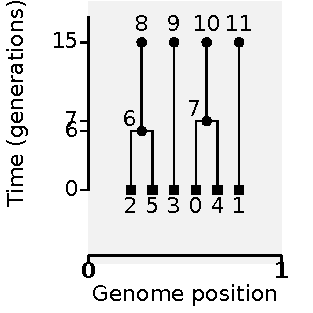
\includegraphics[width=0.48\textwidth]{images/model-duration-and-model-completion.pdf}
\end{center}
\caption{\label{fig:start-duration} DTWF simulations running for 10 generations starting from genertion 5 until genration 15.}
\end{figure}

It is also worth noting that some models, like \texttt{SweepGenicSelection}, are only defined for a specific time interval and do not run until coalescence.

\subsubsection{Multiple models}\label{multiple-models}

Different ancestry models can be combined using \msprime. For example, the DTWF model can be used to simulate the more recent
past, while the faster standard model can be used to simulate the more distant past.

\begin{pythoncode}
ts = msprime.sim_ancestry(
    2, population_size=1000,
    model=[
        msprime.DiscreteTimeWrightFisher(duration=200),
        msprime.StandardCoalescent(),
    ],
    random_seed=2953)
\end{pythoncode}

In this code block, for example, we simulate the coalescent process for two samples under the \emph{DTWF} model for the first 200 generations
and then switch to the \emph{StandardCoalescent} model for the remaining generations. Figure \ref{fig:polytomy} shows the tree
simulated by this example; we can see a polytomy (where three lineages coalesce at the same time), which could not occur under the
\emph{StandardCoalescent} model.

\begin{figure}
\begin{center}
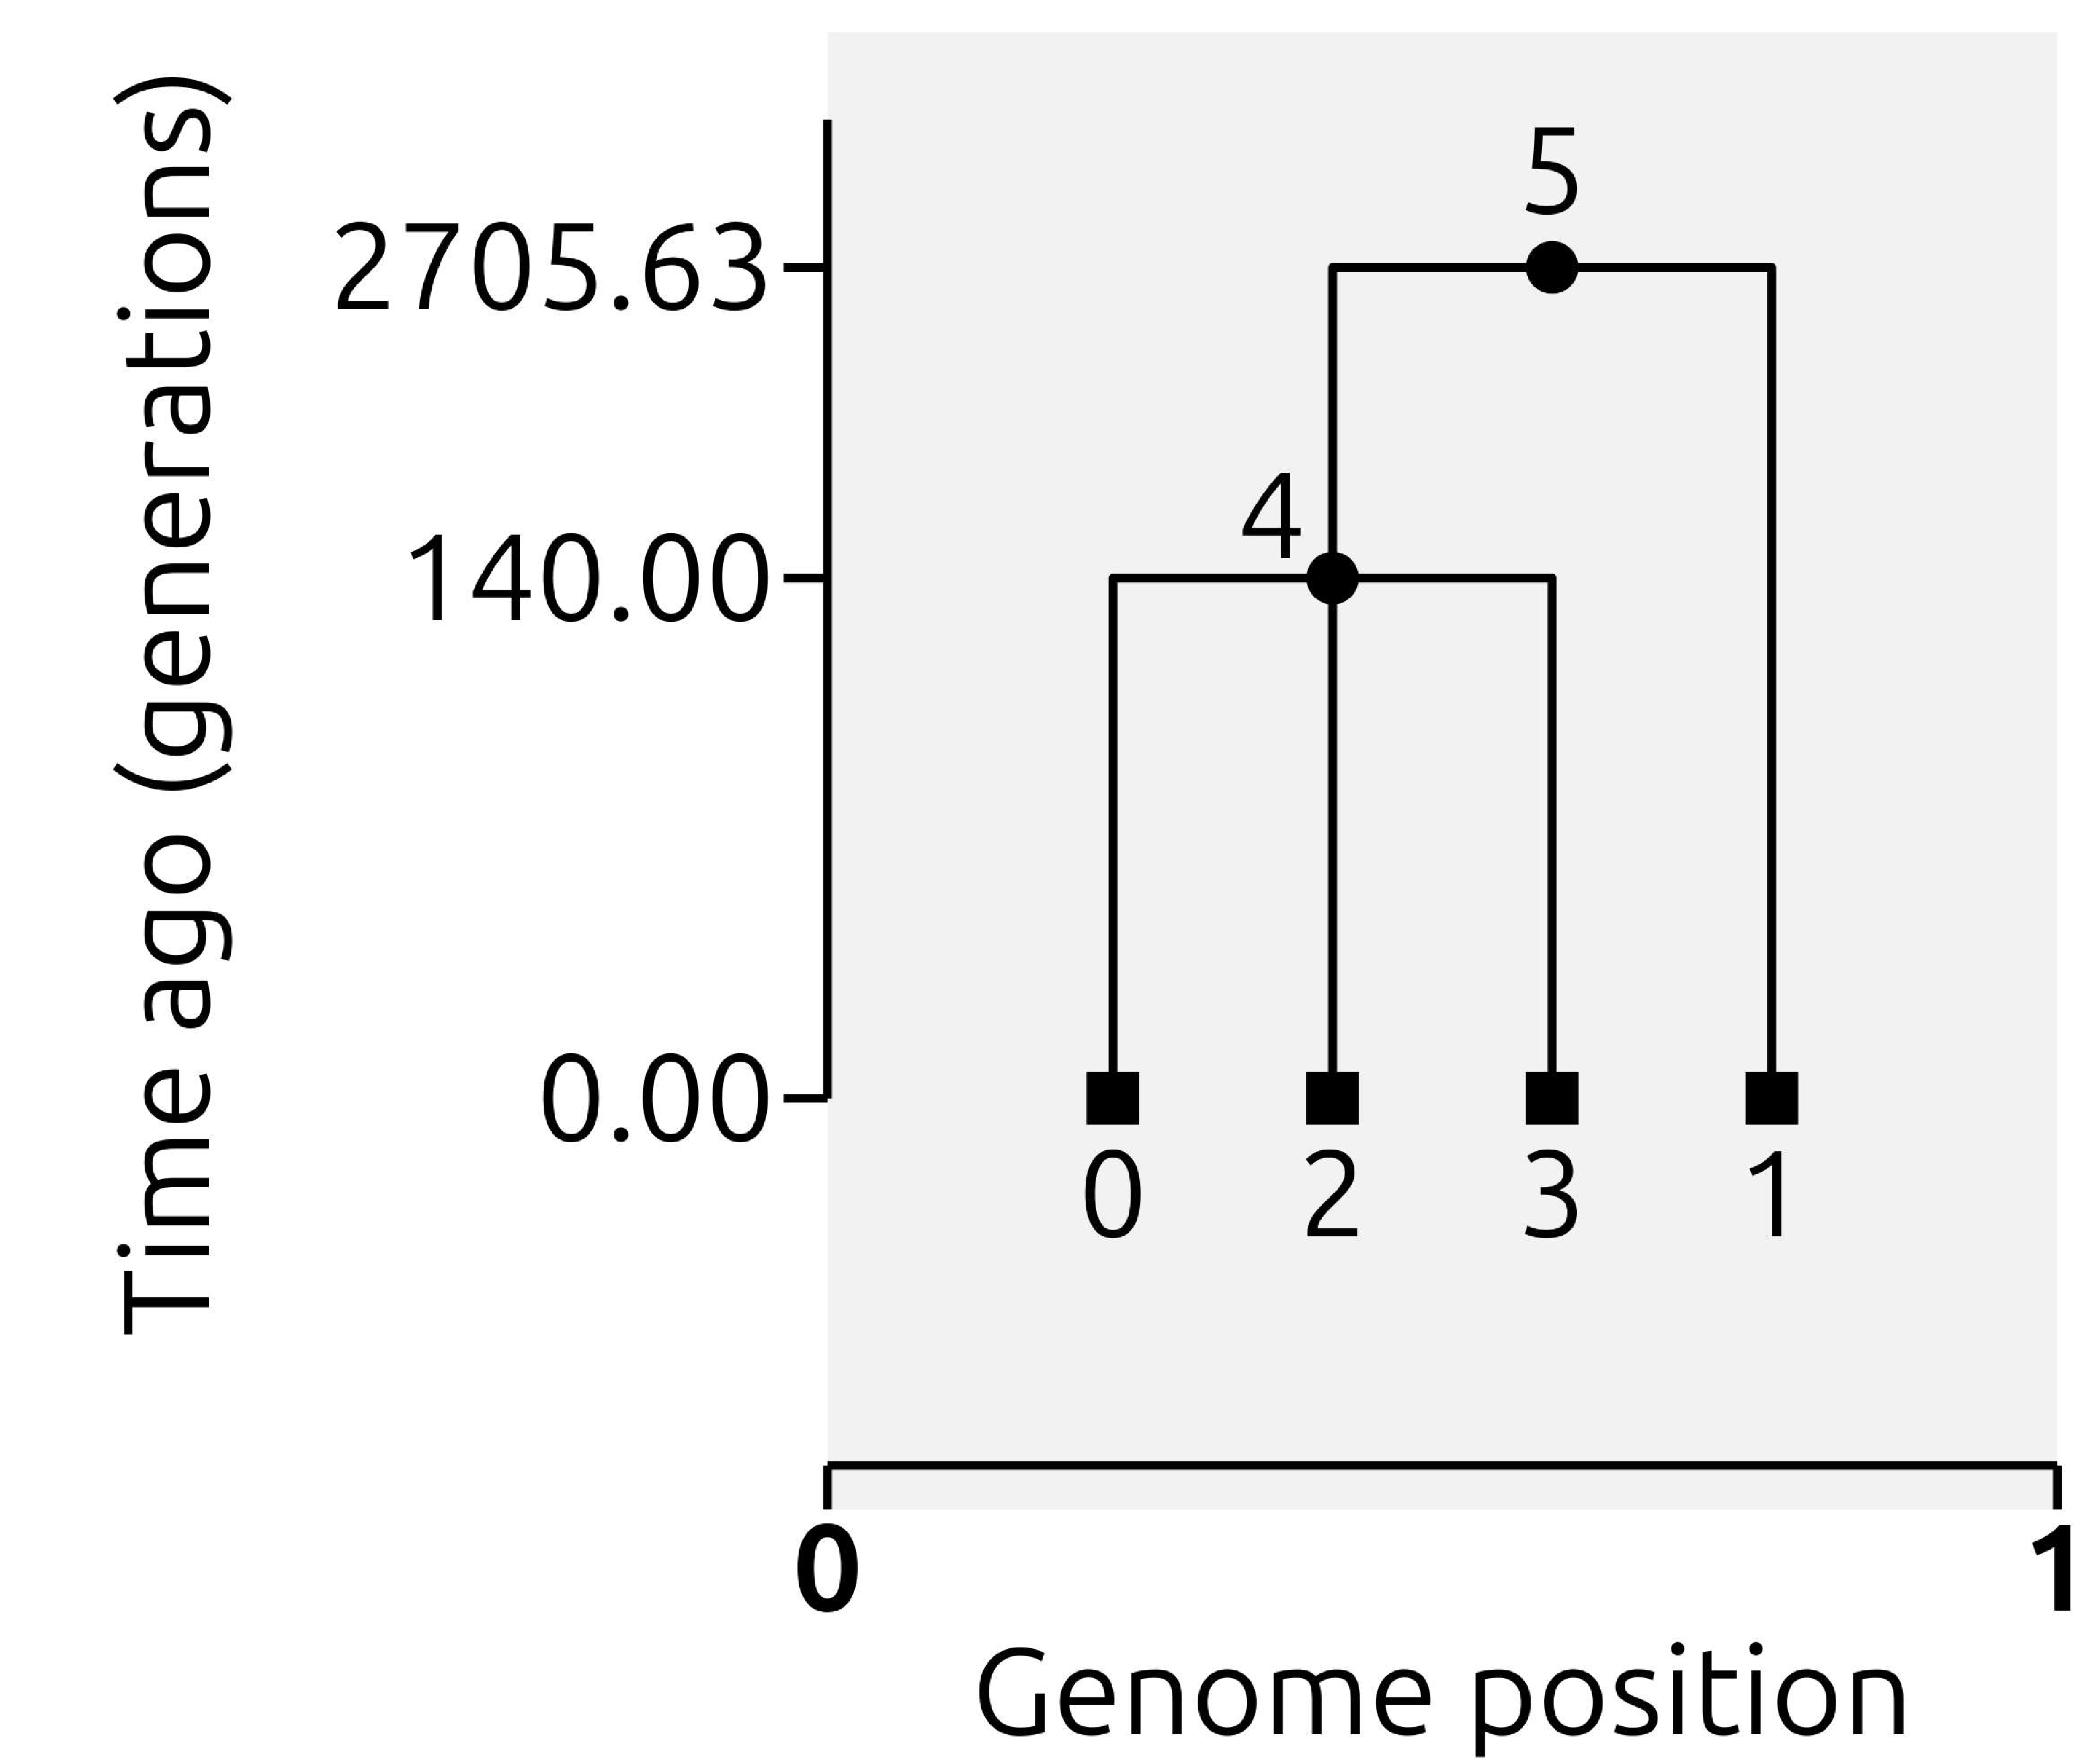
\includegraphics[width=0.48\textwidth]{images/polytomy.pdf}
\end{center}
\caption{\label{fig:polytomy} Tree simulated with a combination of the \emph{DTWF} model and a \emph{StandardCoalescent} model. Polytomy is observed.}
\end{figure}

\runinhead{Selective sweeps}\

Selective sweeps are usually simulated using a combination of the selective sweep model that runs for a specific
period and a neutral model (usually the standard coalescent model) that runs until coalescence. In this example,
we will do a simple selective sweep simulation.

\begin{pythoncode}
L = 1e6  # Length of simulated region
Ne = 1e3
sweep_model = msprime.SweepGenicSelection(
    position=L / 2,  # middle of chrom
    start_frequency=1.0 / (2 * Ne),
    end_frequency=1.0 - (1.0 / (2 * Ne)),
    s=0.25, dt=1e-6)
\end{pythoncode}

In the above code block, we defined a hard sweep on the middle position of a 1 megabase region. This sweep starts with a frequency of \(1/(2*N_e)\) and
until it almost reaches fixation. We set the selection coefficient to be 0.25 and dt, which is the small increment of time for stepping through the sweep
phase of the model, to be 1e-6.

Running the simulation is rather simple, as shown in the following code block:

\begin{pythoncode}
msprime.sim_ancestry(
    5,
    model=[sweep_model,
           msprime.StandardCoalescent()],
    population_size=Ne, recombination_rate=1e-7,
    sequence_length=L)
\end{pythoncode}

This code block simulates the coalescent process for 5 samples using the selective sweep model and then runs the standard coalescent model until
coalescence.

\subsubsection{Fixed pedigree}\label{fixed-pedigree}

A pedigree records the ancestry relationships between individuals, which can limit the possibilities of genetic inheritance. It is possible to
simulate ancestry conditioned on a fixed pedigree using \msprime\ by using the \texttt{FixedPedigree} model. This model limits the transfer of
genetic material from ancestors to descendants while still allowing for recombination. Recombination events occur randomly; therefore, each of
the ancestor's diploid genomes is a mixture of the genomes of their parents defined by the pedigree.

Pedigree can be recorded as a string, where each line contains the ID of the node, the ID of the first parent, the ID of the
second parent, the time of this node, and whether the node is a sample node. The following example visualises a sample pedigree.

\begin{pythoncode}
import io
ped_txt = """\
# id parent0 parent1 time is_sample
0   5   4   0.0 1
1   3   3   0.0 1
2   3   4   0.0 1
3   7   7   1.0 0
4   8   8   1.0 0
5   8   6   1.0 0
6   9   10  2.0 0
7   10  10  2.0 0
8   9   9   2.0 0
9   11  12  3.0 0
10  11  12  3.0 0
11  .   .   4.0 0
12  .   .   4.0 0
"""
pedigree = msprime.parse_pedigree(io.StringIO(ped_txt), sequence_length=100)
\end{pythoncode}

This pedigree is visualised in Figure~\ref{fig:pedigree}.

\begin{figure}
\begin{center}
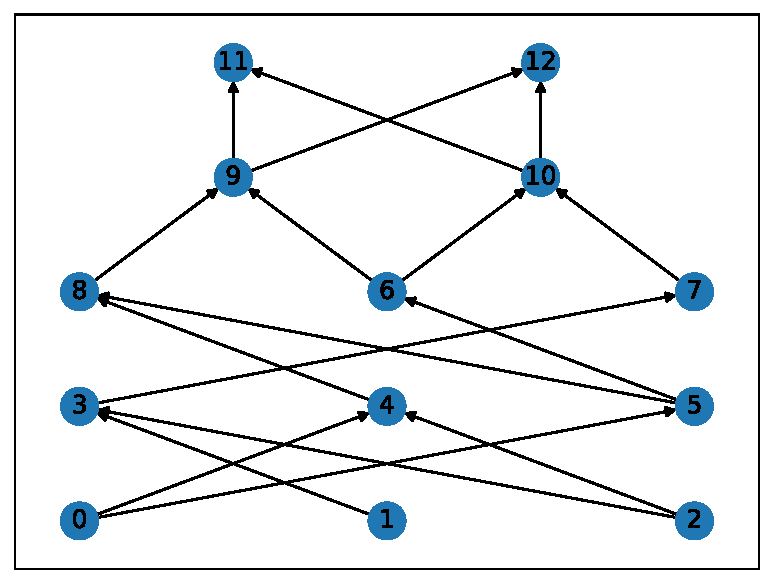
\includegraphics[width=0.48\textwidth]{images/pedigree.pdf}
\end{center}
\caption{\label{fig:pedigree} A visualised pedigree.}
\end{figure}

In the following code block, this pedigree is used to simulate ancestry using the \texttt{FixedPedigree} model.

\begin{pythoncode}
ped_ts = msprime.sim_ancestry(
    initial_state=pedigree, model="fixed_pedigree",
    random_seed=41, recombination_rate=0.001)
node_labels = {node.id: f"{node.individual}({node.id})"
    for node in ped_ts.nodes()}
\end{pythoncode}

The result of the simulation is shown in Figure~\ref{fig:pedigree-simulation}, where the node labels show the individual ID and the node ID;
 because of recombination, the result is two trees for the same fixed pedigree.

\begin{figure}
\begin{center}
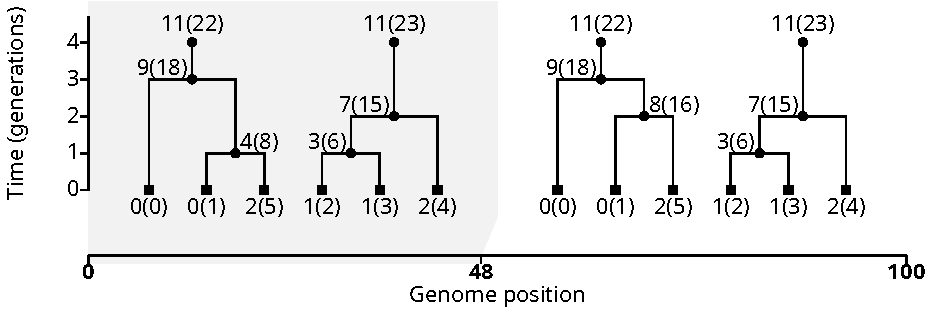
\includegraphics[width=0.75\textwidth]{images/pedigree-simulation.pdf}
\end{center}
\caption{\label{fig:pedigree-simulation} Tree visualisation of ancestory simulations conditioned on a fixed pedigree.}
\end{figure}


%%%%%%%%%%%%%%%%%%%%%%%%%%%%%%%%%%%

\section{Processing results}\label{processing-results}

In the previous section we showed how to run simulations in \msprime, and
how to construct population models and demographic histories. In this
section we show how to process the results of simulations. This is not a
comprehensive review of the capabilities of the \msprime\ Python API, but
concentrates on some useful examples.
\msprime\ is specifically designed to enable very large simulations, and
the processing methods we demonstrate below are all very efficient. To
illustrate this, we consider a simulation of 200,000 samples of 10 megabases
from a simple two-population model with human-like parameters:

\begin{pythoncode}
demography = msprime.Demography.isolated_model([2*(10**4)]*2)
demography.add_migration_rate_change(
    time=50000, source=1, dest=0, rate=1.0)

ts = msprime.sim_ancestry(
    samples={0: 10**5, 1: 10**5},
    demography=demography, recombination_rate=1e-8,
    sequence_length=10*10**6, random_seed=3, ploidy=1)

ts = msprime.sim_mutations(
    ts, rate=1e-8, random_seed=7, discrete_genome=False)
print((ts.num_trees, ts.num_sites))

>>> (93844, 102270)
\end{pythoncode}

This simulation required about 20 seconds to complete. Note that we set the
\texttt{discrete\_genome} parameter of the \texttt{sim\_mutations} method to
\texttt{False} to simulate mutations using an infinitely many sites model.
We will leverage the features of this model, where identical by state
mutations are identical by descent, to compute summary statistics.


\subsection{Computing MRCAs}\label{computing-mrcas}

We are often interested in finding the most recent common ancestor (MRCA)
of a pair (or many pairs) of samples. For example, identity-by-descent
(IBD) tracts are defined as contiguous stretches of genome in which the
MRCA for a pair of samples is the same. Computing IBD segments for a
pair of samples is very straightforward:

\begin{pythoncode}
def ibd_segments(ts, a, b):
    trees_iter = ts.trees()
    tree = next(trees_iter)
    last_mrca = tree.mrca(a, b)
    last_left = 0
    segment_lengths = []
    for tree in trees_iter:
        mrca = tree.mrca(a, b)
        if mrca != last_mrca:
            left = tree.interval[0]
            segment_lengths.append(left - last_left)
            last_mrca = mrca
            last_left = left
    segment_lengths.append(ts.sequence_length - last_left)
    return np.array(segment_lengths) / ts.sequence_length

sns.histplot(
    ibd_segments(ts, 0, 1), label="Within population", kde=True)
sns.histplot(ibd_segments(ts, 0, 10**5),
    label="Between populations", kde=True)
plt.xlim(-0.0001, 0.003)
plt.legend()
plt.ylabel("Count")
plt.xlabel("Fraction of genome length");
\end{pythoncode}

\begin{figure}
\begin{center}
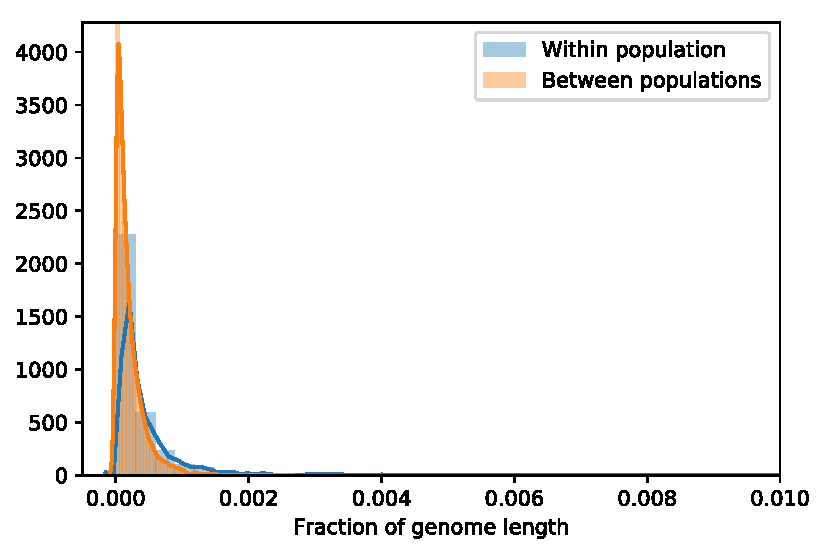
\includegraphics[width=\textwidth]{images/plot_12.pdf}
\end{center}
\caption{\label{fig:ibd_segments} The distribution of the length of IBD
segments for a pair of samples taken from the same or different populations.}
\end{figure}

In this example we create a function \texttt{ibd\_segments} that returns
a NumPy array of the lengths of IBD segments for a given pair of
samples, \texttt{a} and \texttt{b}. It works simply by computing the
MRCA for the samples at the left hand side of the sequence and then,
moving rightwards, records a segment each time the MRCA changes. We then
plot the distribution of tract lengths for samples 0 and 1 (which are
both in population 0), and also the tract lengths for a pair of
samples from different populations. The results are shown in
Figure~\ref{fig:ibd_segments}. As we might expect, the tract
lengths are shorter for the between population pair.

Of course, we would need to sample many such pairs of samples or longer sequences to get a reasonable approximation of the real distribution of block lengths.
Because the main cost of this function is the iteration over all the
trees in the sequence, it would be more efficient to keep track of the MRCAs
for different pairs in a single iteration rather than repeatedly
call the above \texttt{ibd\_segments} function.

\subsection{Sample counts}\label{sample-counts}

The \msprime\ API provides an extremely efficient way to count the number of samples that are beneath a particular node in a tree. This can be used,
for example, to compute allele frequencies efficiently and is the basis
for many of the fast algorithms in the API. As a simple illustration of
this technique, consider the following code to compute the number of
sites with derived allele frequency less than 1\%:

\begin{pythoncode}
N = ts.num_samples
threshold = 0.01
num_rare_derived = 0
for tree in ts.trees():
    for site in tree.sites():
        assert len(site.mutations) == 1
        mutation = site.mutations[0]
        if tree.num_samples(mutation.node) / N < threshold:
            num_rare_derived += 1
print((num_rare_derived, num_rare_derived / ts.num_sites))

>>> (65292, 0.635241236391232)
\end{pythoncode}

    In this example we iterate over all the trees in the tree sequence, and
then iterate over all the sites in each tree. We find the frequency
of the derived allele at each site using the \texttt{num\_samples}
method, which returns the number of samples subtending a given
node. The underlying implementation ensures that this operation requires
constant time, and so it is \emph{very} efficient. We see that such rare alleles are common.
(Since we are using the infinitely many sites model, we can be confident that
each mutation occurs at a unique site. Using other mutation models may produce
tree sequences with back or recurrent mutations, where this simple approach
will not work. To emphasise this point and to ensure that
the above code chunk is not accidentally applied in such sitations, we have included an
\texttt{assert} statement. We use asserts in a similar way in later code chunks.)

A powerful feature of this sample-counting approach is that we can
perform the same operation over an arbitrary subset of the samples. For
example, suppose we wished to count the number of sites that are private
to a specific population:

\begin{pythoncode}
def num_private_sites(pop_id):
    pop_samples = ts.samples(pop_id)
    num_private = 0
    for tree in ts.trees(tracked_samples=pop_samples):
        for site in tree.sites():
            assert len(site.mutations) == 1
            mutation = site.mutations[0]
            total = tree.num_samples(mutation.node)
            within_pop = tree.num_tracked_samples(mutation.node)
            if total == within_pop:
                num_private += 1
    return num_private

private_0 = num_private_sites(0)
private_1 = num_private_sites(1)
print((ts.num_sites, private_0 + private_1, private_0, private_1))

>>> (102783, 102117, 50850, 51267)
\end{pythoncode}

    This example is very similar, except we provide an extra argument to
\texttt{ts.trees}. The \texttt{tracked\_samples} argument specifies a list of samples to be tracked, which can be
any arbitrary subset of the samples in the simulation. Here we indicate
that we are interested in tracking the set of samples within the
population in question. Again, we iterate over all trees and over all
sites within trees. Then, for each infinite sites mutation we
compute two frequencies: the overall number of samples that inherit from
the mutation's node, and the number of tracked samples \emph{within the focal
population} that inherit from this node. If the total count is
equal to the within-population count, we know that this mutation is private to the population.

\subsection{Obtaining subsets}\label{obtaining-subsets}

In some situations it is useful to analyse data for different subsets of
the samples separately. This is possible using the \texttt{simplify}
method:

\begin{pythoncode}
samples = [1, 3, 5, 7]
ts_subset = ts.simplify(samples)
print(
    ts_subset.num_sites, ts_subset.num_trees,
    ts.num_sites, ts.num_trees)
>>> (11925, 5323, 102783, 93598)
\end{pythoncode}

Here we extract the tree sequence representing the history of a tiny
subset of the original samples, with IDs 1, 3, 5 and 7. The subset tree
sequence contains all the genealogical information relevant to the
subsamples, but no more. Concretely, both coalescences that are not ancestral to the
subsample and coalescences that predate
the MRCA of the subsample are excluded. Thus, the number of distinct trees is greatly
reduced. By default, we also remove any sites that have no mutations
within these subtrees (i.e., those that are fixed for the ancestral
state). These can be retained by using the
\texttt{filter\_zero\_mutation\_sites=False} argument.

Node IDs in the simplified tree sequence are not the same as in the
original. The \texttt{map\_nodes} argument allows us to obtain the
mapping from IDs in the original tree sequence to their equivalant nodes
in the new tree sequence.

\begin{pythoncode}
ts_subset, node_map = ts.simplify(samples, map_nodes=True)
tree = ts_subset.first()
node_labels = {
    node_map[j]: "{}({})".format(node_map[j], str(j))
    for j in range(ts.num_nodes)}
tree.draw_svg(node_labels=node_labels)
\end{pythoncode}

\begin{figure}[t]
\centering
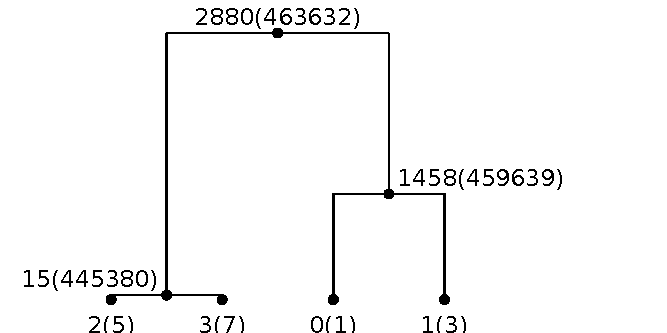
\includegraphics[width=0.48\textwidth]{images/plot_13.pdf}
\caption{\label{fig-tree-subset} Tree of a subset of the samples in a large
simulation. Node IDs in the subset and full tree sequences are shown.}
\end{figure}

The result of running this code chunk is show in Figure~\ref{fig-tree-subset}.
Here we draw the first tree in the subset tree sequence, showing the new
node IDs along with the IDs from the original tree sequence in
parentheses. The number of nodes is greatly reduced from the original.

\subsection{Processing variants}\label{processing-variants}

While it is nearly always more efficient to work with mutations in terms
of their context within the trees, it is sometimes more convenient to
work with the allelic states of the samples. This information is
obtained in msprime using the \texttt{variants()} iterator, which
returns a \texttt{Variant} object for each site in the tree sequence. A
\texttt{Variant} consists of: (a) a reference to the \texttt{Site} in question;
(b) the \texttt{alleles} at this site (the strings representing the
actual states); and (c) the \texttt{genotypes} representing the observed
state for each sample. The \texttt{genotypes} are encoded in a NumPy
array, such that \texttt{variant.alleles{[}variant.genotypes{[}j{]}{]}}
gives the allelic state for sample ID \texttt{j}. The values in the
\texttt{genotypes} array are therefore indexes into the \texttt{alleles}
list. The ancestral state at a given site is guaranteed to be the first
element in the \texttt{alleles} list, but no other assumptions about
ordering of the alleles list should be made.

For biallelic sites, working with genotypes is straightforward as the
genotypes array can only contain 0 and 1 values, which correspond to
the ancestral and derived states, respectively. The \texttt{genotypes}
values are returned as a NumPy array, and so the full NumPy library is
available for efficient processing. As an example, we show here how to
count the number of sites at which the derived allele is at frequency
less than 10\%. Using the genotypes in this way is convenient, as
complex patterns of back and recurrent mutations can be handled without
difficulty.

\begin{pythoncode}
%%time
threshold = 0.1
num_rare = 0
for variant in ts.variants():
    # Will work for any biallelic sites;
    # back/recurrent mutations OK
    assert len(variant.alleles) == 2
    if np.sum(variant.genotypes) / ts.num_samples < threshold:
        num_rare += 1
print(num_rare)
>>> 83757
CPU times: user 1min 30s, sys: 4 ms, total: 1min 30s
\end{pythoncode}

This code is straightforward, as we simply iterate over all variants and
count the number of 1 values in the genotypes array. Using the \texttt{np.sum}
function, this operation is efficient. Generating all the genotypes for
200,000 samples at 100,000 sites, however,
is an expensive operation and the overall calculation takes about 1.5 minutes
to complete.

In the case of infinite sites mutations, we can recast this operation
to use the efficient sample counting methods describe in
Section~\ref{sample-counts}. This approach is far more
efficient, requiring less than 2 seconds to compute the same value.
\begin{pythoncode}
%%time
num_rare = 0
for tree in ts.trees():
  for site in tree.sites():
    # Only works for infinite sites mutations.
    assert len(site.mutations) == 1
    mutation = site.mutations[0]
    if tree.num_samples(mutation.node)/ts.num_samples<threshold:
        num_rare += 1
print(num_rare)
>>> 83757
CPU times: user 1.75 s, sys: 36 ms, total: 1.79 s
\end{pythoncode}

\subsection{Incremental calculations}\label{incremental-calculations}

A powerful property of the tree sequence representation is that we can
efficiently find the differences between adjacent trees. This is very
useful when we have some value that we wish to compute that changes in a
simple way between trees. The \texttt{edge\_diffs} iterator provides us
with the information that we need to perform such incremental
calculations. Here we use it to keep a running track of the total branch
length of our trees, without needing to perform a full traversal each
time.

\begin{pythoncode}
def get_total_branch_length(ts):
  current = 0
  total_branch_length = np.zeros(ts.num_trees)
  for j, (_, edges_out, edges_in) in enumerate(ts.edge_diffs()):
    for e in edges_out:
        current -= ts.node(e.parent).time-ts.node(e.child).time
    for e in edges_in:
        current += ts.node(e.parent).time-ts.node(e.child).time
    total_branch_length[j] = current
  return total_branch_length
\end{pythoncode}

    This function returns the total branch length value for each tree in the
sequence as a NumPy array. It works by keeping track of the total branch
length as we proceed from left to right, and storing this value in the
output array for each tree. The \texttt{edge\_diffs} method returns a
list of the edges that are removed for each tree transition
(\texttt{edges\_out}) and a list of edges that are inserted
(\texttt{edges\_in}). Computing the current value for the total branch
length is then simply a case of subtracting the branch lengths for all
outgoing edges and adding the branch lengths for all incoming edges.
This is extremely efficient because, after the first tree has been
constructed there is at most four incoming and outgoing edges~\citep{kelleher2016efficient}. Thus,
each tree transition costs \emph{constant time}.

\begin{pythoncode}
%%time
tbl = get_total_branch_length(ts)

CPU times: user 7.67 s, sys: 64 ms, total: 7.74 s
\end{pythoncode}

In contrast, if we compute the total branch length by performing a
full traversal for each tree, each tree transition is very costly
when we have a large sample size. In this example, computing the array of branch lengths
using the incremental approach given here took 8 seconds. Computing the
same array using the \texttt{tree.total\_branch\_length} for each tree
in a straightforward way still had not completed after \emph{twenty
minutes}. (This is because \msprime\ currently implements this operation
by a full traversal in Python; in future this may change to using the
algorithm given here.) Full tree traversals of large trees are
expensive, and great gains can be made if calculations can be expressed
in an incremental manner using \texttt{edge\_diffs}.


\subsection{Exporting variant data}\label{exporting-variant-data}

If the \msprime\ API doesn't provide methods to easily calculate the
statistics you are interested in, it's straightforward to export the
variant data into other libraries using the \texttt{genotype\_matrix()}
or \texttt{variants()} methods. We recommend the excellent
\texttt{scikit-allel}~\citep{miles2017scikit} and
\texttt{pylibseq} [\url{https://pypi.python.org/} \url{pypi/pylibseq}],
libraries (\texttt{pylibseq} is a Python interface to
\texttt{libsequence}~\citep{thornton2003libsequence}). If you wish to export data to
external programs, VCF may be best option, which is supported using the
\texttt{write\_vcf} method. The \texttt{simplify} method is useful here
if you wish to export data from a subset of the simulated samples.

However, it is worth noting that for large sample sizes, exporting
genotype data may require a great deal of memory and take some time. One
of the advantages of the \msprime\ API is that we do not need to
explicitly generate genotypes in order to compute many
statistics of interest.

\section{Validating analytic predictions}\label{validating-analytical-predictions}

In this section we show some examples of validating simple analytic
predictions from coalescent theory using simulations. The number of
segregating sites is the total number of mutations that occurred in the
history of the sample (assuming the infinite sites mutation model).
Since mutations happen as a Poisson process along the branches of the
tree, what we are really interested in is the distribution of the total
branch length of the tree. The results in this section are well known
classical results from coalescent theory; this section is intended as a
demonstration of how to proceed when comparing analytic results to
simulations. We show some idiomatic examples for integrating with
the state-of-the-art data analysis packages such
as Pandas~\citep{mckinney2010data} and Seaborn~\citep{michael_waskom_2017_883859}.
All analytic predictions are taken from \cite{wakely2008coalescent}.

\subsection{Total branch length and segregating sites}
The first properties we are interested in are the mean and the
variance of the total branch length of coalescent trees. (Note that, as
before, we set \emph{ploidy=1} to convert between \msprime's default diploid time
scaling to the haploid time scaling of these analytic results.)

\begin{pythoncode}
ns = np.array([5, 10, 15, 20, 25, 30])
num_reps = 10000
n_col = np.zeros(ns.shape[0] * num_reps)
T_total_col = np.zeros(ns.shape[0] * num_reps)
row = 0
for n in ns:
    for ts in msprime.sim_ancestry(n, population_size=1,
            num_replicates=num_reps, ploidy=1):

        tree = ts.first()
        n_col[row] = n
        T_total_col[row] = tree.total_branch_length
        row += 1
df = pd.DataFrame({"n": n_col, "T_total": T_total_col})
\end{pythoncode}

    We first create an array of the six different \(n\) values that we wish to simulate, and then create arrays to hold the results of the
simulations. Because we are running 10,000 replicates for each sample
size, we allocate arrays to hold 60,000 values. This approach of storing
the data in arrays is convenient because it allows us to use Pandas
dataframes in an idiomatic fashion. We then iterate
over all of our sample sizes and run 10,000 replicates of each. For each
simulation, we simply store the sample size value and the total branch
length in a Pandas dataframe. This gives us access to many powerful data analysis tools (including the Seaborn library, which we use for visualisation here).

After we have created our simulation data, we define our analytic
predictions and plot the data.

\begin{pythoncode}
def T_total_mean(n):
    return 2 * np.sum(1 / np.arange(1, n))

def T_total_var(n):
    return 4 * np.sum(1 / np.arange(1, n)**2)

mean_T = np.array([T_total_mean(n) for n in ns])
stddev_T = np.sqrt(np.array([T_total_var(n) for n in ns]))
ax = sns.violinplot(
    x="n", y="T_total", data=df, color="grey", inner=None)
ax.plot(mean_T, "-");
ax.plot(mean_T - stddev_T, "--", color="black");
ax.plot(mean_T + stddev_T, "--", color="black");
group = df.groupby("n")
mean_sim = group.mean()
stddev_sim = np.sqrt(group.var())
x = np.arange(ns.shape[0])
ax.plot(x, mean_sim, "o")
line, = ax.plot(x, mean_sim - stddev_sim, "^")
ax.plot(x, mean_sim + stddev_sim, "^", color=line.get_color());
\end{pythoncode}

% \begin{figure}
% \begin{center}
%     \parbox{5cm}{
%     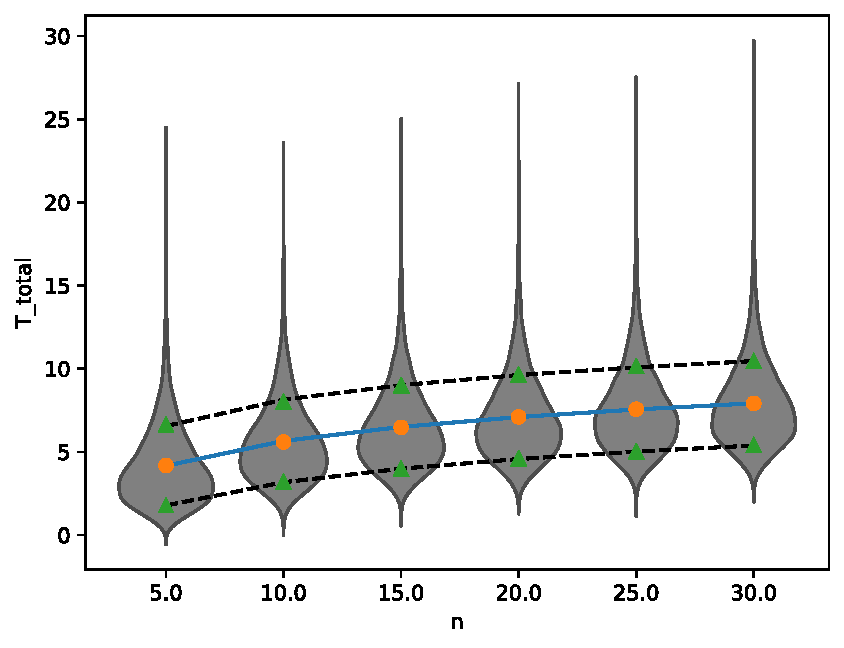
\includegraphics[width=5cm]{images/plot_14.pdf}
%     \begin{center}(A)\end{center}
%     }%
%     \qquad
%     \parbox{5cm}{
%     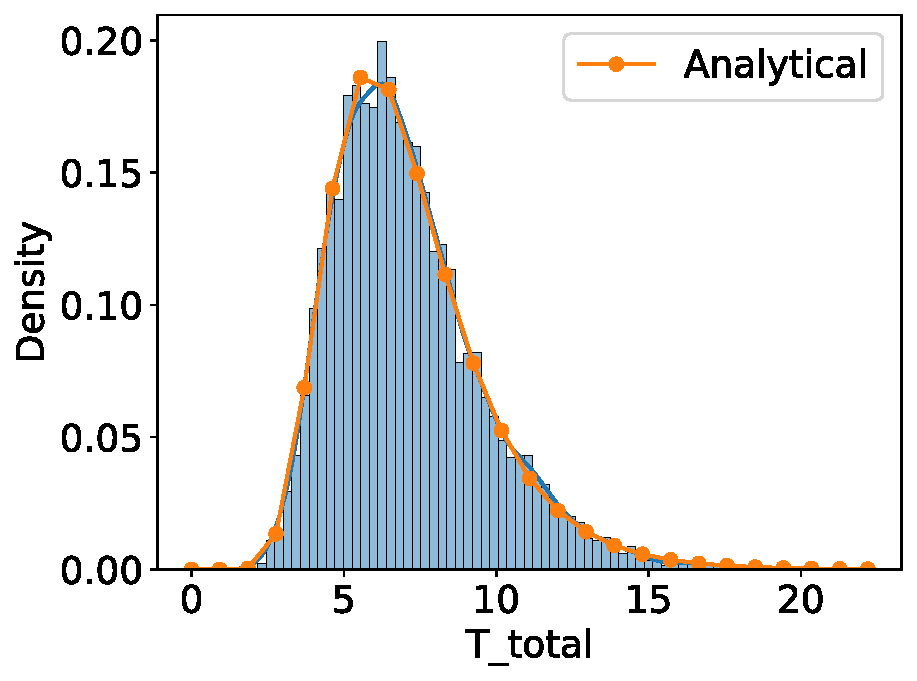
\includegraphics[width=5cm]{images/plot_15.pdf}
%     \begin{center}(B)\end{center}
%     }
%     \caption{Comparisons of the distribution of simulated total branch lengths
%         with analytic results. (A) The full distribution of simulated
%         values (violin plots) along with observed and predicted mean and
%         standard deviations for a range of sample sizes. (B) The full
%         simulated and predicted distribution of total branch lengths
%         for $n = 20$.}
%     \label{fig:segsites-norecomb}
% \end{center}
% \end{figure}

\begin{figure}[t]
\centering
\subfloat[][
The full distribution of simulated
values (violin plots) along with observed and predicted mean and
standard deviations for a range of sample sizes.
]{
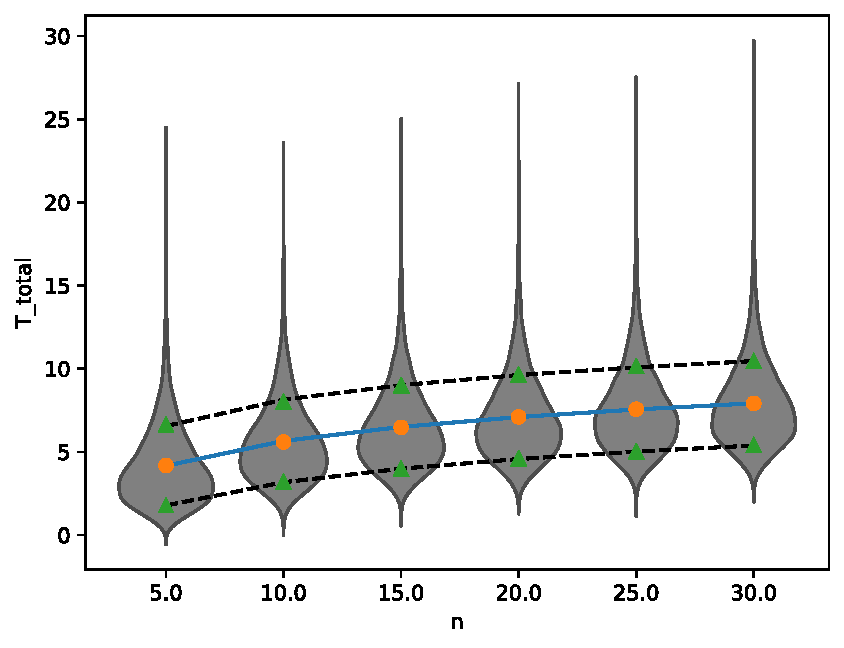
\includegraphics[width=0.75\textwidth]{images/plot_14.pdf}
\label{fig-segsites-norecomb-a}}
\qquad\qquad
\subfloat[][
The full simulated and predicted distribution of total branch length for $n = 20$.
]{
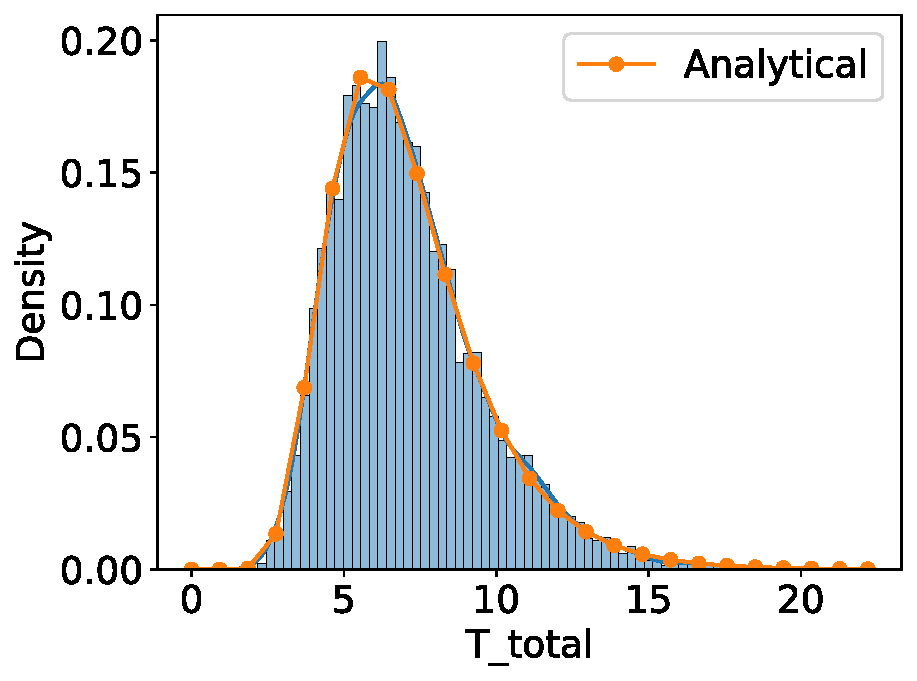
\includegraphics[width=0.75\textwidth]{images/plot_15.pdf}
\label{fig-segsites-norecomb-b}}
\caption{\label{fig-segsites-norecomb}
Comparisons of the distribution of simulated total branch lengths
with analytic results.
}
\end{figure}

    The plot in Figure~\ref{fig-segsites-norecomb-a} shows the simulated
distribution of the total branch length
over replicate simulations (each violin is a distribution for a given
sample size). We also show our analytic prediction for the mean and
variance of each distribution (the dashed lines show +/- one standard
deviation from the mean). Also shown are the observed means and standard
deviations from the simulations, as green circles and red triangles,
respectively. We can see that the simulated values match our theoretical
predictions for mean and variance very well. We can also see, however,
that these one-dimensional summaries of the distribution capture some
essential properties but lose some important aspects of the
distribution.

    Ideally, we wish to capture the full distribution analytically. In the following code chunk we define the analytic
prediction for the total branch length distribution, and compare it with the simulated distribution for a sample of size 20. The results are shown in
Figure~\ref{fig-segsites-norecomb-b}. We can see an excellent agreement between
the smoothed kernel
density estimate produced by Seaborn and the theoretical prediction.

\begin{pythoncode}
def T_total_density(n, t):
    e_t2 = np.exp(-t / 2)
    return 0.5 * (n - 1) * e_t2 * (1 - e_t2)**(n - 2)

n = 20
T_total_20 = T_total_col[n_col == n]
ts = np.linspace(0, np.max(T_total_20), 25)
t_densities = np.array([T_total_density(n, t) for t in ts])
sns.histplot(T_total_20, kde=True, stat="density")
plt.plot(ts, t_densities, marker="o", label="Analytical")
plt.xlabel("T_total")
plt.legend();
\end{pythoncode}

Since we cannot directly observe branch lengths, we are usually more
interested in mutations when working with data. The mutation process is
intimately related to the distribution of branch lengths, since
mutations occur randomly along tree branches. One simple summary of the
mutational process is the total number of segregating sites, that is, the number of
sites at which we observe variation. We can obtain this very
easily from simulations simply by specifying a mutation rate parameter.
(Note again that we set \emph{ploidy = 1} and our mutation rate
\(= \theta / 2\) in order to convert to \msprime's time scales.)

\begin{pythoncode}
def S_dist(n, theta, k):
    S = 0
    for i in range(2, n + 1):
        S += ((-1)**i * scipy.special.binom(n - 1, i - 1)
            * (i - 1) / (theta + i - 1)
            * (theta / (theta + i - 1))**k)
    return S

n = 20
theta = 5
num_replicates = 1000
simulation = np.zeros(num_replicates)
replicates = msprime.sim_ancestry(
    n, population_size=1, num_replicates=num_replicates, ploidy=1)
for j, ts in enumerate(replicates):
    ts = msprime.mutate(ts, rate=theta/2)
    simulation[j] = ts.num_sites  # number of seg. sites
ks = np.arange(np.max(simulation))
analytical = np.array([S_dist(n, theta, k) for k in ks])
sns.histplot(simulation, kde=True, stat="density")
plt.plot(ks, analytical, marker='o', label="Analytical")
plt.xlabel("Segregating sites")
plt.legend();
\end{pythoncode}

\begin{figure}[t]
\centering
\subfloat[][
    The distribution of the number
    of segregating sites for $n=20$, $\theta=5$ and no recombination
    over 1000 simulation replicates, along with analytic prediction.]{
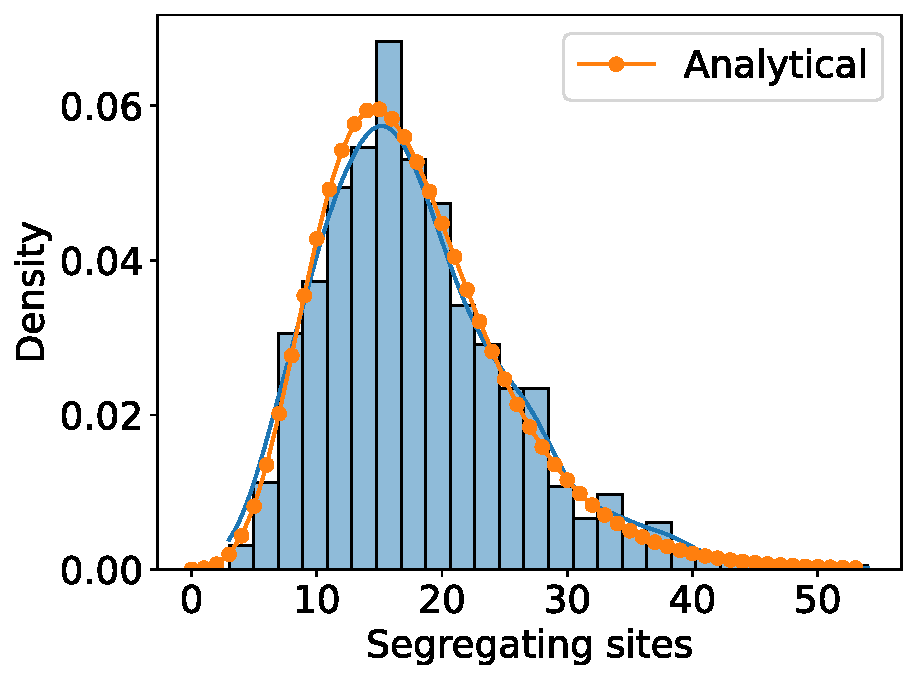
\includegraphics[width=0.75\textwidth]{images/plot_16.pdf}
\label{fig-segsites-a}}
\qquad\qquad
\subfloat[][
    The mean and variance of the number of segregating sites
    over 10000 simulation replicates with $n=2$, $\theta=2$ and
    varying recombination rate, along with analytic predictions.]{
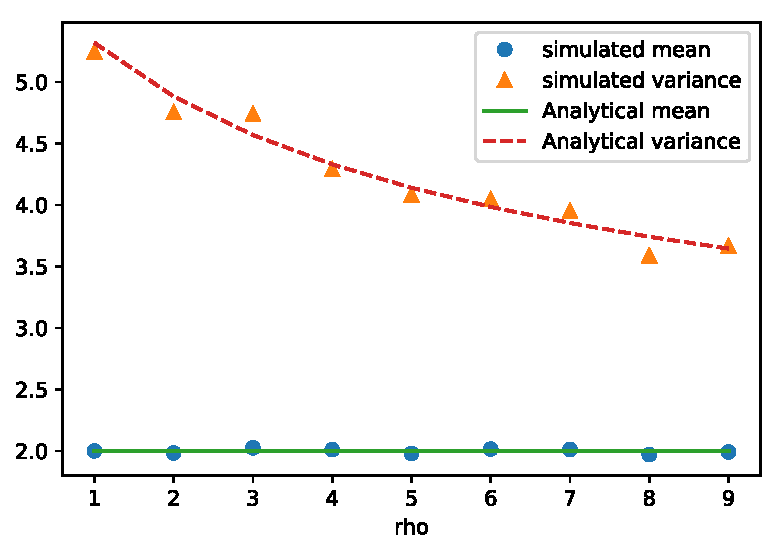
\includegraphics[width=0.75\textwidth]{images/plot_17.pdf}
\label{fig-segsites-b}}
\caption{\label{fig-segsites}
Simulations of the number of segregating sites, and
comparisons with analytic predictions.
}
\end{figure}

Here we take 1000 replicate simulations, store the number of infinite
sites mutations for each and plot this distribution in
Figure~\ref{fig-segsites-a}. Also plotted is the analytic prediction, which again provides an excellent fit.


\subsection{Recombination}

In the previous section we saw how to run simulations to generate trees
under the assumptions of the single-locus coalescent and compare these
with analytic predictions. This assumes that our data is not affected
by recombination, which is often unrealistic. Here we show how to
compute empirical distributions of equivalent quantities, and compare
these with classical results from the literature. Since analytic
results for many quantities are generally unknown for the case of recombination along a linear sequence, we limit ourselves to the pairwise samples.

\begin{pythoncode}
theta = 2
num_replicates = 10000
rhos = np.arange(1, 10)
N = rhos.shape[0] * num_replicates
rho_col = np.zeros(N)
s_col = np.zeros(N)
row = 0
for rho in rhos:
    replicates = msprime.sim_ancestry(
        2, num_replicates=num_replicates, ploidy=1,
        recombination_rate=rho/2, population_size=1,
        discrete_genome=False, sequence_length=1)

    for ts in replicates:
        ts = msprime.sim_mutations(
            ts, rate=theta/2, discrete_genome=False)
        rho_col[row] = rho
        s_col[row] = ts.num_sites
        row += 1
df = pd.DataFrame({"rho": rho_col, "s": s_col})
\end{pythoncode}

In this code chunk we again run $10^4$ replicate simulations for a range
of input parameters, and store the results in a Pandas data frame. We
are interested in the effects of recombination rate in this example,
and so the parameter that we vary is the scaled recombination rate
$\rho$ (noting, again, that we set \emph{ploidy = 1} and
\texttt{recombination\_rate} = $\rho / 2$ to convert to \msprime's
time scales).

\begin{pythoncode}
def pairwise_S_mean(theta):
    return theta
def f2(rho):
    return (rho + 18) / (rho**2 + 13 * rho + 18)
def pairwise_S_var(theta, rho):
    integral = scipy.integrate.quad(lambda x: (rho-x)*f2(x),0,rho)
    return theta + 2 * theta**2 * integral[0] / rho**2

group = df.groupby("rho")
plt.plot(group.mean(), "o", label="simulated mean")
plt.plot(group.var(), "^", label="simulated variance")
plt.plot(
    rhos, [pairwise_S_mean(theta) for rho in rhos], "-",
    label="Analytical mean")
plt.plot(rhos, [pairwise_S_var(theta, rho) for rho in rhos], "--",
label="Analytical variance")
plt.xlabel("rho")
plt.legend();
\end{pythoncode}

After defining our analytic predictions for the mean and variance of the
number of segregating sites, we then plot the observed and predicted values
in Figure~\ref{fig-segsites-b}.
Comparing the simulated results to analytic predictions we see
excellent agreement. The mean number of segregating sites is not
affected by recombination, but recombination does substantially reduce
the variance.

\section{Example inference scheme}\label{sec:inference}

    The analytical challenges of deriving likelihood functions even under
highly idealized models of population structure and history have led to
the development of likelihood-free inference methods, in particular
Approximate Bayesian Computation (ABC)~\citep{Beaumont2002}.
ABC approximates the posterior distribution of model parameters by drawing from
simulations. Because of its flexibility ABC has become a standard
inference tool in statistical population genetics \citep[see][for a review]{csillery2010approximate}.
We will demonstrate how \msprime\ can be used to set up an ABC inference
by means of a simple toy example. We stress that this is meant as an
illustration rather than a inference tool for practical use. However,
given the flexibility of \msprime, it should be
relatively straightforward to implement more a realistic framework focused
on specific inference applications.

We assume that data for 200 loci or sequence blocks (these could be RAD
loci in practice) for a single diploid individual have been generated
from each of two populations. We would like to infer the amount of gene
flow between the two populations. For the sake of simplicity we will
assume the simplest possible model of population structure; that is, two
populations, of the same effective size exchanging migrants at a
constant rate of $m$ migrants per generation.

The function \texttt{run\_sims} simulates a dataset consisting of a
specified number of loci (\texttt{num\_loci}) given a migration rate
\(M\). We generate a single dataset of 50 loci assuming a migration rate
\(M=0.3\) migrants per generation, which we will use as a (pseudo)observed dataset in the ABC
implementation.

\begin{pythoncode}
nsamp = 2
theta = 2
true_m = 0.3
num_loci = 200

def run_sims(m, num_loci=1, theta=0):
    demography = msprime.Demography.island_model(
        [1, 1], migration_rate=m)
    replicates = msprime.sim_ancestry(
        {0: nsamp, 1:nsamp}, demography=demography,
        num_replicates=num_loci, ploidy=1,
        discrete_genome=False, sequence_length=1)
    for ts in replicates:
        yield msprime.sim_mutations(
            ts, rate=theta, discrete_genome=False)

def get_joint_site_frequency_spectra(reps):
    data = np.zeros((num_loci, nsamp + 1, nsamp + 1))
    for rep_index, ts in enumerate(reps):
        data[rep_index] = ts.allele_frequency_spectrum([
            [0, 1], [2,3]], polarised=True)
    return data

truth = get_joint_site_frequency_spectra(
    run_sims(true_m, num_loci=num_loci, theta=2))
\end{pythoncode}

    The \texttt{run\_sims} function returns an iterator with the complete
tree sequence and mutational information of each locus. We use the
function \texttt{get\_joint\_site} \texttt{\_frequency\_spectra} to summarize the
polymorphism information as the joint site frequency spectrum (jSFS) of
each locus, i.e. the blockwise site frequency spectrum
or bSFS \cite[sensu][]{Lohse2016}.
Note that higher level population genetic summaries, e.g.\ pairwise
measures of divergence and diversity such as \(D_{XY}\) \citep{Nei1972} and
\(F_{ST}\)~\citep{wright1950genetical} or multi-population \(F\)
statistics~\citep{Durand2009,patterson2012ancient} which are often
used in ABC inference are just further (and lossy) summaries of the jSFS.

Since \msprime\ simulates rooted trees, the columns and rows
of the unfolded jSFS correspond to the frequency of derived mutations in
each population and the entries of the jSFS are simply mutation counts.
E.g.\ for the first locus we have:
\begin{pythoncode}
print(truth[0])

>>> [[ 0.  14.  0.]
     [ 0.  0.  0.]
     [ 8.  1.  0.]]
\end{pythoncode}

    One could base inference on the bSFS \citep{Lohse2016, Beeravolu2017}, but we will for the sake of simplicity use a simpler (and lossy)
summary of the data: the average jSFS across loci. For analyses based on
SNPs, it is convient to normalize the jSFS by the total number of
mutations:
\begin{pythoncode}
truth_mean = np.mean(truth, axis=0)
truth_mean /= np.sum(truth_mean)
print(truth_mean)

>>> [[0.         0.24496958 0.16471689]
     [0.20846982 0.05662143 0.06948994]
     [0.16752457 0.08820777 0.        ]]
\end{pythoncode}

    To illustrate a simple ABC inference, we will focus on a single
parameter of interest, the migration rate \(M\).
ABC measures the fit of data simulated under the prior to the observed
data via a vector of summary statistics. We will use the jSFS as a
summary statistic and approximate the jSFS for each \(M\) value as the
mean length of genealogical branches across 100 simulation replicates (\texttt{num\_reps}). Below we
draw 10,000 \(M\) values from the prior and use the functions
\texttt{run\_sims} and \texttt{approx\_jSFS} to approximate the jSFS for
 replicate. We assume an exponential distribution, a common choice of prior \citep{hey2004multilocus}.

\begin{pythoncode}
import tskit

num_reps = 100
num_prior_draws = 10000
prior_m = np.random.exponential(0.1, num_prior_draws)
def approx_jSFS(m):
    reps = run_sims(m, num_loci=num_reps)
    B = np.zeros((num_reps, nsamp + 1, nsamp + 1))
    for rep_index, ts in enumerate(reps):
        B[rep_index] = ts.allele_frequency_spectrum(
            [[0,1],[2,3]], mode='branch',
            polarised=True, span_normalise=False)
    data = np.mean(B, axis=0)
    return data / np.sum(data)

with cf.ProcessPoolExecutor(max_workers=4) as executor:
    futures = [
        executor.submit(approx_jSFS, prior) for prior in prior_m]
    prior_jSFS = np.array([
        f.result() for f in cf.as_completed(futures)])

print(prior_jSFS[0])
\end{pythoncode}

Here we run 100 simulation replicates for each of the 10,000
$m$ values drawn from the prior, giving a total of 1 million individual simulations.
We use the \texttt{concurrent.futures} module to distribute these
computations over the available CPU cores.

Once this has completed, we compute the Euclidean distance between the estimated branch-jSFS for each
draw from the prior (\texttt{prior\_jSFS}) and the site-jSFS in the (pseudo)observed
data (\texttt{truth\_mean}), as both values should be
similar~\citep{ralph2020efficiently}.
\begin{pythoncode}
distances = np.zeros(num_prior_draws)
for j in range(num_prior_draws):
    distances[j] = np.sqrt(np.sum((prior_jSFS[j]-truth_mean)**2))
\end{pythoncode}

\begin{figure}[t]
\centering
\subfloat[][
Prior and posterior ABC distributions
and estimated 95\% approximate credible interval.
]{
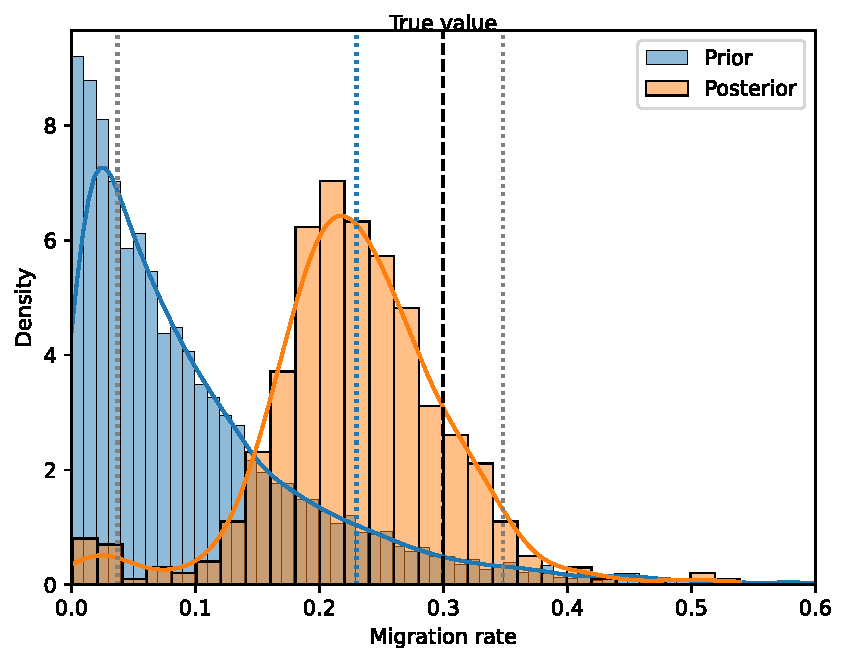
\includegraphics[width=0.75\textwidth]{images/plot_18.pdf}
\label{fig-abc-a}}
\qquad\qquad
\subfloat[][
Mean and root-mean-square-error of migration rate estimates computed
from pseudo-observed data sets.]{
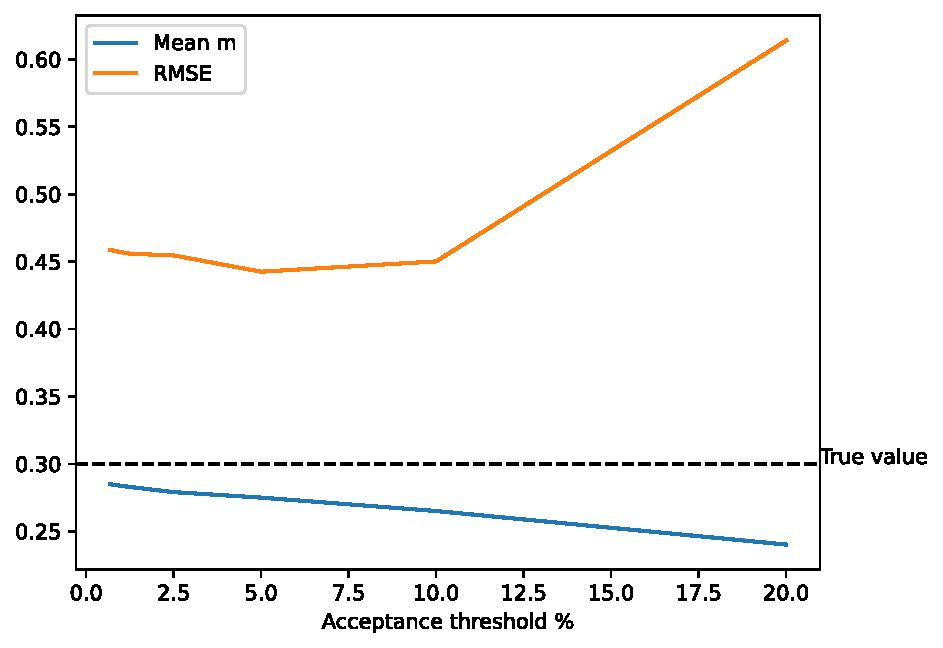
\includegraphics[width=0.75\textwidth]{images/plot_20.pdf}
\label{fig-abc-b}}
\caption{\label{fig-abc}ABC results.}
\end{figure}

% \begin{figure}
% \begin{center}
%     \parbox{5cm}{
%     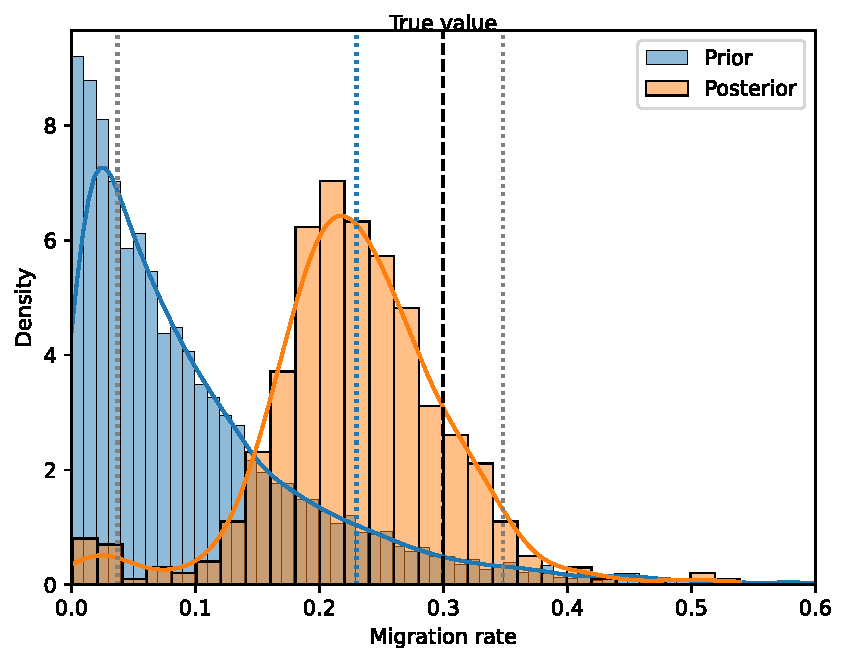
\includegraphics[width=5cm]{images/plot_18.pdf}
%     \begin{center}(A)\end{center}
%     }%
%     \qquad
%     \parbox{5cm}{
%     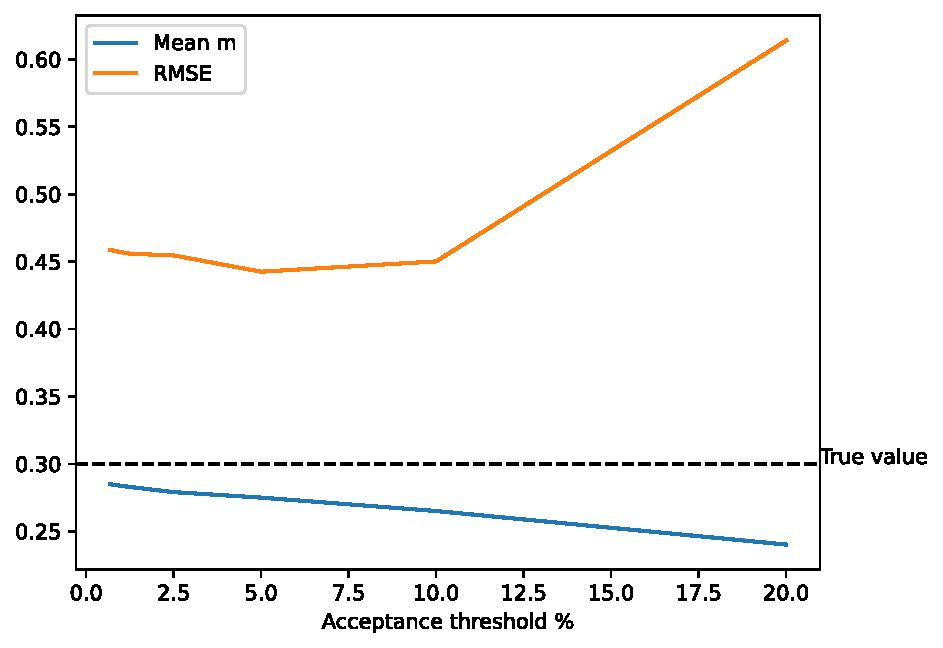
\includegraphics[width=5cm]{images/plot_20.pdf}
%     \begin{center}(B)\end{center}
%     }
%     \caption{ABC results. (A)  Prior and posterior ABC distributions
%     and estimated 95\% approximate credible interval.
%     (B) Mean and root-mean-square-error of
%     migration rate estimates computed from pseudo-observed data sets.}
%     \label{fig:abc}
% \end{center}
% \end{figure}

    In its simplest form, ABC approximates the posterior by sampling from
the simulated data via an acceptance threshold. Here we approximate the
posterior distribution of \(m\) using the 5\% of simulation replicates
that most closely match the average jSFS of the observed data.
Figure~\ref{fig-abc-a} shows that the posterior
distribution (shown in green) is centred around \(m=0.25\).
\begin{pythoncode}
cutoff = np.percentile(distances, 5)
keep = np.where(distances < cutoff)
post_m = prior_m[keep]
mean_m = np.mean(post_m)
ci_m = np.percentile(post_m, 2.5), np.percentile(post_m, 95.75)
sns.histplot(prior_m, label="Prior", kde=True, stat="density")
sns.histplot(post_m, label="Posterior", kde=True, stat="density")
\end{pythoncode}

The mean and the 95\% approximate posterior credible interval for \(m\)
are:
\begin{pythoncode}
print([mean_m, ci_m])

>>> [np.float64(0.2706689107323255),
    (np.float64(0.1680558635307605),
     np.float64(0.40359485279569585))]
\end{pythoncode}


Although the true value of \(m=0.3\) is contained within the 95 \% credible interval, the posterior distribution is clearly downwardly biased. This bias is in fact expected given that our prior is also strongly biased towards low \(m\). We can check the effect the acceptance threshold on the inference and get a sense of the expected information about \(m\) using a cross-validation procedure: we repeat the inference on pseudo-observed data sets (PODS) simulated under a known truth. Since we can re-use the same set of replicates simulated under the prior for inference, such cross-validation is computationally efficient.

Figure~\ref{fig-abc-b} shows the mean and the root mean square error (RMSE) of \(m\) estimates (across 100 PODS) against the acceptance threshold and confirms that both the downward bias in \(m\) estimates and the associated RMSE increase with larger acceptance tresholds. While this toy example illustrates the principle of ABC inference, sampling only a small fraction of simulations generated under the prior is clearly computationally inefficient and more efficient sampling strategies for ABC inference have been developed \citep{Beaumont2002}. In practice, we are generally interested in fitting parameter-rich models and it would be straightforward to implement ABC inference for complex model of population structure and demography in \msprime.

\section{Discussion}
\label{sec:discussion}
\texttt{Msprime} simulates the complete history of a sample of genomes under
the influence of recombination. Although there has been some confusion about 
the precise meaning of the term, the recent consensus has been to loosely 
refer to such structures as Ancestral Recombination Graphs, or
ARGs~\citep{wong2024general}. Since \msprime\ was first released in 2014
there has been an explosion of interest in ARGs, with four separate 
review articles published in 2024~\citep{brandt2024promise,
lewanski2024era,nielsen2024inference,wong2024general}. 
This has largely been
driven by exciting developments in inference, with great strides being
made in both statistically rigorous Bayesian sampling 
approaches~\citep{rasmussen2014genome,mahmoudi2022bayesian,deng2024robust} 
and large-scale hueristic
methods~\cite{speidel2019method,kelleher2019inferring,
zhang2023biobank,gunnarsson2024scalable},
their potential combination~\citep{bisschop2025likelihoods},
along with important auxiliary inference tasks such as node
dating~\cite{wohns2022unified,deng2025general}.
Sophisticated simulation tools, however, have also played an important
role. The ability to generate truth data at scale 
under a range of complex demographic
models~\citep{adrion2020stdpopsim,gower2022demes,lauterbur2023expanding}
and arbitrary patterns of
selection~\citep{kelleher2018efficient,haller2018tree,gower2025accessible}
is critical to evaluate these inference methods.
\texttt{Msprime} is likely to continue playing a significant role 
in this ongoing ARG revolution.

\section*{Acknowledgments}

We would like to thank Simon Aeschbacher for comments on the ABC inference example,
and to thank Yan Wong, Joseph Marcus and Julien Dutheil for
detailed and insightful feedback.
JK acknowledges EPSRC (research grant EP/X024881/1),
NIH (research grants HG011395 and HG012473)
and the Robertson Foundation.
KL []
% JK is supported by Wellcome Trust grant 100956/Z/13/Z to Gil McVean.
% KL is supported by an Independent Research fellowship from the Natural Environment Research Council (NE/L011522/1).

\section*{Online resources}

\begin{tabular}{ll}
Jupyter notebook & \url{https://github.com/jeromekelleher/spg-chapter} \\
Documentation & \url{https://tskit.dev/msprime/docs/} \\
GitHub & \url{https://github.com/tskit-dev/msprime} \\
Tskit & \url{https://tskit.dev/} \\
Tskit documentation & \url{https://tskit.dev/tskit/docs/stable/} \\
Tskit tutorials & \url{https://tskit.dev/tutorials} \\
\end{tabular}

\bibliography{references}

\end{document}
